% \documentclass[sigconf]{acmart}
% \documentclass[acmtog,anonymous,nonacm,review]{acmart}
\documentclass[acmtog, nonacm]{acmart}
\acmSubmissionID{1154}
\citestyle{acmauthoryear}
% \citestyle{plain}
\settopmatter{printacmref=true}
\usepackage{subcaption}

% remove SIGGRAPH information
% \settopmatter{printacmref=false} % Removes citation information below abstract
% \renewcommand\footnotetextcopyrightpermission[1]{} % removes footnote with conference information in first column
% \pagestyle{plain} % removes running headers

\makeatletter
\let\@authorsaddresses\@empty
\makeatother
\setcopyright{none}
\settopmatter{printacmref=false} % Removes citation information below abstract
\renewcommand\footnotetextcopyrightpermission[1]{}% removes footnote with conference information in first column


\usepackage[ruled]{algorithm2e} % For algorithms
% \usepackage{xr} % to cross reference with supplement
% \externaldocument[supp-]{7Suppl_text}
\usepackage{multicol}

\renewcommand{\algorithmcfname}{ALGORITHM}
\SetAlFnt{\small}
\SetAlCapFnt{\small}
\SetAlCapNameFnt{\small}
\SetAlCapHSkip{0pt}

% \acmJournal{TOG}

%fix errors with overrightarrow
\DeclareRobustCommand*{\ora}{\overrightarrow}


\begin{document}
	% \title{Inaccurate Distance Estimation in Head-Mounted Displays}
    % \title{Perceived Distance Errors in Head-Mounted Displays}
    %\title{Perceptual Impacts of Inaccurate Stereo Geometry in VR}
    \title{Perceptual Sensitivity to Stereo Geometry Errors in Head-Mounted Displays}
	\author{Raffles Xingqi Zhu}
	\affiliation{
			\institution{Reality Labs Research, Meta}
   			\country{USA}
                \institution{McGill University}
                \country{Canada}
		}
			\email{raffles.zhu@mail.mcgill.ca}

	\author{Charlie S. Burlingham}
	\affiliation{
			\institution{Reality Labs Research, Meta}
   			\country{USA}
		}
	\email{cburlingham@meta.com}
   
	\author{Olivier Mercier}
	\affiliation{
			\institution{Reality Labs Research, Meta}
   			\country{USA}
		}
	\email{omercier@meta.com}

	\author{Phillip Guan}
	\affiliation{
			\institution{Reality Labs Research, Meta}
   			\country{USA}
		}
	\email{philguan@meta.com}
        % \renewcommand{\shortauthors}{Kwak, Penner, Wang, Saeedpour-Parizi, Mercier, Wu, Murdison, and Guan}
	
	\begin{abstract}
        Virtual and augmented reality head-mounted displays (HMDs) render and display head-tracked, stereo images to create an egocentric, 3D percept to the viewer. Errors in stereo geometry introduced by rendering from an incorrect location (e.g., from tracking errors) or viewing from the wrong position (e.g., from fitment errors) can alter the depth and distance a user perceives compared to the intended geometry. In this work we evaluate how accurately a purely geometric framework that models distance misperception arising from inaccurate stereo geometry can predict changes to user reach behavior. We show that some stereo geometry errors can induce both under- and over-reaching, and the magnitude of error is consistent with geometric predictions. Surprisingly, we find the mismatches between HMD display separation and viewer interpupillary distance error have significantly less impact on reach behavior than predicted by geometry prediction. In a follow-up psychophysical study we find a relatively large detection threshold ($\approx$6 mm) to mismatches between viewer interpupillary distance and headset display separation, confirming the reaching result. We additionally show how perceptual thresholds to various stereo geometry errors change with viewing distance and scene complexity.
	\end{abstract}
	% uncomment for submission
        \setcopyright{none}
        \settopmatter{printacmref=false} % Removes citation information below abstract
        \renewcommand\footnotetextcopyrightpermission[1]{}% removes footnote with conference information in first column
 
% \begin{CCSXML}
% 	<ccs2012>
% 	<concept>
% 	<concept_id>10010147.10010371.10010387.10010866</concept_id>
% 	<concept_desc>Computing methodologies~Virtual reality</concept_desc>
% 	<concept_significance>500</concept_significance>
% 	</concept>
% 	</ccs2012>
% \end{CCSXML}
% \ccsdesc[500]{Computing methodologies~Virtual reality}	
% 	\keywords{virtual reality, distance underestimation, rendering errors, world-locked rendering}	
	%% A "teaser" image appears between the author and affiliation
	%% information and the body of the document, and typically spans the
	%% page.

	\begin{teaserfigure}
		\centering
		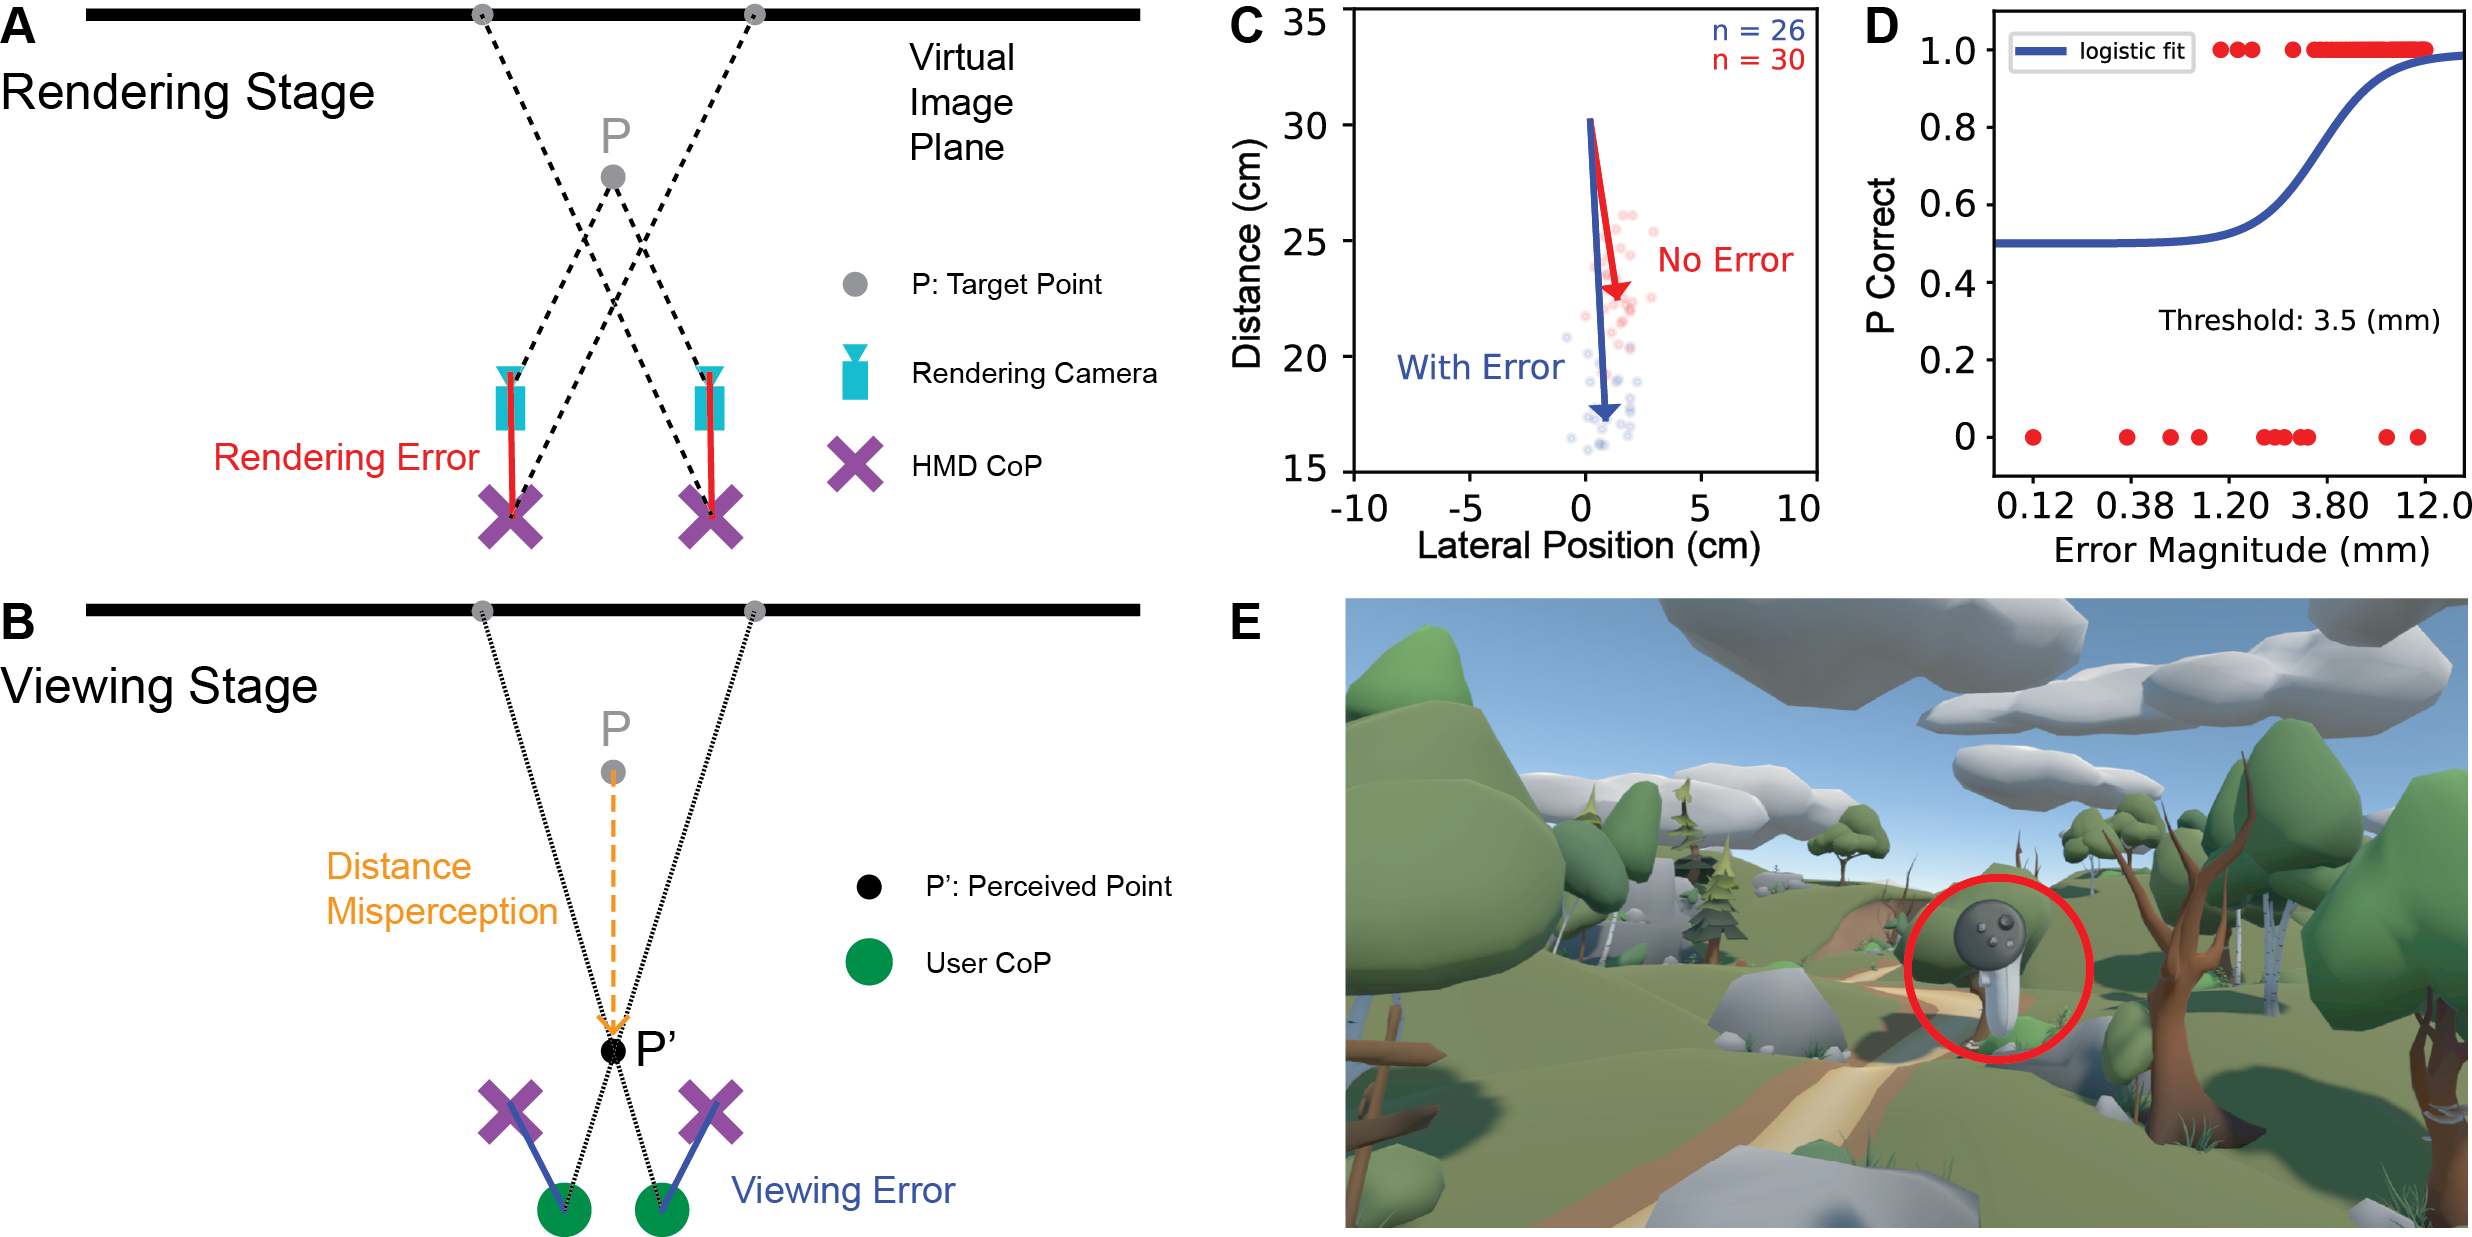
\includegraphics[width=\textwidth]{figures/teaser.png}
        \caption{We investigate whether geometric predictions from purposefully introduced rendering and viewing stereo geometry errors in head-mounted displays (HMDs) accurately model changes in perceived distance when these errors are viewed in an HMD. Some of the errors we examined would traditionally require physically changing the position of an HMD on the user's head (e.g., to simulate changes in eye relief). Precise manipulations of headset fit are difficult in practice, so we built an HMD software platform that allowed us render images in our HMD consistent with making these physical manipulations to facilitate our user studies. The impact of these errors was measured in a series of experiments involving blind reaching and visual only distance discrimination. \textbf{(A)} Rendering errors are displacements of the rendering cameras from the HMD centers of projection (CoP), typically located at the center of the eyebox. In this example, the rendering cameras are too far forward which can occur when video passthrough images are directly streamed to the HMD displays without view reprojection. Here the ray angle from the camera to a target point P is captured by the camera, and this ray is projected onto the display from the HMD CoP leading to the incorrect render geometry (the correct ray should pass from the HMD CoP through the target point P to the display). \textbf{(B)} Independent from rendering errors, viewing errors are displacements of the CoP of the viewer's eyes (user CoP) from the HMD CoP. Here, the incorrectly rendered left and right stereo images from (A) are additionally viewed from an incorrect location. The HMD interaxial distance (IAD, the distance between HMD CoP) is too large relative to the viewer's interpupillary distance (IPD). The viewer's eye relief is also too large, causing their eyes to be behind the HMD CoP. A simple ray-intersection model predicts that the combined effects of rendering and viewing errors will result in a misperception of the black point P' from the intended gray point P. \textbf{(C)} We evaluated the efficacy of this triangulation model in a blind reaching experiment, which required us to first use an eye-tracked HMD to compensate for naturally occurring viewing errors so that we could properly evaluate simulated rendering and viewing errors. This plot shows the blind reach performance for one participant in the no rendering or viewing error condition (red) and when HMD IAD is higher than user IPD (blue). In the absence of error, we find that there is still an under-reaching bias. Removing this bias aligns blind reach distances with predictions of our triangulation model for two out of three error conditions tested. \textbf{(D)} We measured error detection thresholds using a two interval forced choice psychophysical task. This design was made possible by leveraging eye tracking in our HMD platform to compare no-error stereo geometry to perturbed geometry due to introduced rendering and viewing errors. One example participant's binary response data for IPD viewing error are shown in red, with the psychometric function shown in blue. \textbf{(E)} The scene used in our experiments (controller in the reaching experiments is highlighted for emphasis).}
		\label{fig:teaser}
	\end{teaserfigure}
	\maketitle
	% for internal sharing
        %	\pagestyle{plain} % removes running headers
	
	\section{Introduction}
\label{sec:intro}
Precise interaction in head-mounted displays (HMDs) requires correct stereo geometry for users to accurately perceive size and distance in virtual environments. Precisely reproducing this geometry requires co-location of three features: for each eye, the Render Camera Center of Projection (CoP), the HMD Display CoP, and the User’s Eye CoP must be spatially aligned. In practice, this is rarely achieved and  many geometric models have been built by researchers to predict the perceptual consequences that may result from these errors \cite{held2008misperceptions, robinett92, woods93, krajancich2020}.

The stereo-projection pipeline is susceptible to two classes of errors. First, rendering errors arise when the render camera used to generate the scene is displaced from the HMD CoP. Rendering errors are commonly introduced due to inaccuracies in tracking the user's head position \cite{holloway1997} and from motion-to-photon latency \cite{allison1999}. In more recently introduced mixed-reality HMDs with video passthrough, rendering errors can be introduced by the static displacement of the see-through video camera in front of user's eyes \cite{biocca98, Lee13, kuo23}.

Second, viewing errors occur when the rendered image is geometrically correct for a nominal eye position, but the user’s actual eye (more specifically, the CoP of the eye) is displaced from this location \cite{vishwanath05, banks2014camera, held2008misperceptions, guan2023perceptual}. Current HMD optical designs assume a fixed, nominal eye position within the "eyebox" to maximize field of view and minimize distortion. HMDs without eyetracking assume the eye is always at this nominal location \cite{Rong25}. Yet, variance in human facial structure, improper headset fit, or mismatches between the headset’s inter-axial distance (IAD) and the user’s interpupillary distance (IPD) inevitably place the user’s Eye CoP away from the Display CoP. Even dynamic factors, such as the movement of the Eye CoP during eye rotations (i.e., ocular parallax), introduce transient viewing errors that most current rendering pipelines ignore \cite{holloway1997, rolland04, wann95}. These displacements fundamentally alter the triangulation geometry of the viewed image that should, according to projective geometry, disrupt the viewer's perception of size and distance.

  
While the theoretical distortions resulting from these rendering and viewing errors can be modeled using stereo geometry, the predictive accuracy of a simple triangulation model remains an open question. Can human perception be predicted simply from first-order geometry, or does the visual system employ higher-order perceptual mechanisms to normalize the percept? Assessing the predictive power of these geometric models is difficult, as manipulating parameters like headset fit, tracking accuracy, and latency are often difficult or infeasible to readily adjust in real headsets.

In this work, we evaluate whether a simple geometric model can predict perceptual responses to errors in stereo geometry. To explore this, we make the following contributions:

\begin{itemize}   
    \item We build a software platform that allows direct manipulation of rendering and viewing errors in a real headset thereby enabling precise and repeatable adjustments of viewing errors without the need to physically manipulate headset fit. We used this platform to conduct a series of user studies and compared these results to the theoretical geometric model, and we additionally provide a web application that can be used to explore these geometric predictions interactively.

    \item  We show that direct passthrough rendering errors and eye relief viewing errors induce changes in reach behavior that are well-predicted by stereo geometry, but we also identify a significant deviation in the case of IPD mismatch, which has a surprisingly small impact compared to model predictions.
    
    \item We conduct a psychophysical experiment exploring perceptual sensitivity to direct passthrough and IPD errors. We find that sensitivity varies with viewing distance and scene content, and confirm a surprising tolerance to IPD errors ($\approx$ 6 mm), even at near distances.
    
    
\end{itemize}


% Our results demonstrate a complex relationship between geometry and perception. We show that Rendering Errors (such as those in direct passthrough) and Eye Relief errors induce distance misperceptions that are tightly predicted by the triangulation model, supporting the hypothesis of geometric determinism. However, we also identify a significant deviation in the case of IPD mismatch, where users exhibit a surprisingly high perceptual tolerance, suggesting that the visual system is not a purely passive receiver of geometric data but possesses specific compensatory plasticity for biological variance. This work provides a rigorous geometric foundation for understanding distance perception in VR, moving the field beyond historical generalizations of underestimation toward a precise, computable model of stereoscopic error.

	\section{Related Work}
\label{sec:related_work}

\paragraph{Distance Underestimation in HMDs}
Over the past several decades many studies have found that distances are underestimated in virtual reality (VR) \cite{creem-regehr_chapter_2015, el_jamiy_distance_2019, el_jamiy_survey_2019, renner_perception_2013}. A variety of theories have been proposed to explain this phenomenon, but a comprehensive explanation has not been found \cite{creem2023perceiving}. Proposed theories on the underlying cause of systematic distance underestimation in HMDs are typically related to effects of HMD hardware, such as field of view (FOV) \cite{kline_distance_1996,buck_comparison_2018}, weight \cite{willemsen_effects_2009,buck_comparison_2018,masnadi_field_2021,masnadi_effects_2022}, display resolution \cite{thompson_does_2004,kelly2022distance,ryu_influence_2005}, and higher-order perceptual effects like scene complexity, realism, presence, and embodiment \cite{el_jamiy_distance_2020,bodenheimer_perceiving_2023,vaziri_impact_2017, gonzalez2019individual}. In a meta analysis, Kelly~\shortcite{kelly2022distance} found that distance is more accurately estimated in newer HMDs. Kelly explored the impact of technical characteristics like FOV and resolution on the magnitude of underestimation across studies, but there are other improvements in newer hardware that are more difficult to quantify such as more accurate head tracking, reduced distortion from improved optical designs, and better fitment systems. These advancements all improve the underlying stereo projection and relatively little work has investigated the effect low-level errors in stereo geometry may have on distance perception in HMDs. Our work is the first to explicitly measure how errors in stereo geometry affect behavior (reaching) which may offer new insights on topics like distance underestimation.

\paragraph{Reaching Experiments in Personal Space}
There are fewer studies on distance estimation in VR for personal space (<2 meters) compared to action space (2-30 meters). Results are mixed showing overestimation \cite{rolland_towards_1995}, underestimation \cite{napieralski_near-field_2011}, and accurate estimation \cite{naceri_depth_2011}. Similar to studies in action space, distance is typically measured using open-loop motor tasks such as blind reaching/pointing or verbal reports. Napieralski et. al \shortcite{napieralski_near-field_2011} found the difference between measurement protocal (blind reaching vs. verbal response) is much greater than the difference between VR and the real world (underestimation in both cases). Closed-loop visual feedback has been shown to improve distance judgement accuracy \cite{kelly_recalibration_2014, mohler_influence_2006, altenhoff_effects_2012}, with visual motor re-calibration leading to more accurate reaching \cite{ebrahimi_effects_2014, ebrahimi_carryover_2015}. One challenge in characterizing reach distance in near space is co-registration of the viewer's egocentric coordinate frame and the coordinate frame of the system used to measure reach distance. Our stereo geometry framework in Section~\ref{sec:model} explores how differences in eye relief in particular may introduce discrepancies between how far a user perceives their reach to be and physically measured reach distance by an external observer.

\paragraph{Perceptual Effects of Inaccurate Geometry in HMDs}
Geometric errors have been shown to affect distance perception experimentally, but most studies evaluate engineering-related errors rather than geometric errors explicitly. For example, geometric calibration alleviates distance underestimation in AR \cite{kellner_geometric_2012}. Magnification also causes significant changes in distance judgments \cite{kellner_geometric_2012, kuhl_hmd_2009, zhang_minification_2012, li_effects_2015}. Some studies have examined the impact of mismatched HMD lens interaxial distance (IAD) to the user's IPD and have found that distance perception is minimally impacted by the IAD-IPD mismatch in action space \cite{chakraborty_inter-pupillary_2024,willemsen_effects_2008, hibbard_implications_2020}, likely a result of stereo cues being less accurate at farther distances \cite{mccann_contributions_2018}. \citeN{guan2023perceptual} detection thresholds to eye relief, IPD, and translational viewing errors, but they do not quantify the impact of these thresholds on user behavior or perception. Many computational models have been presented that examine the effects of viewing errors (i.e., displacement of the user CoP from the HMD CoP) \cite{woods93,held2008misperceptions,rolland04}, but fewer have considered the joint effects of simultaneous viewing and rendering errors \cite{holloway1997}. In this work, we complement prior geometric modeling by also pairing geometric predictions with empirical user studies.

%, but not incorrectly calibrating lens distortion\cite{kuhl_hmd_2009}.
% In a theoretical analysis, \cite{hibbard_implications_2020} showed a mismatched interpupillary distance (IPD) would cause inaccurate depth judgement, particularly that smaller (larger) IPD leads to overestimation (underestimation). 

% Here we propose a first-principles based framework that is applicable to all egocentric display architectures relying on stereoscopic perspective projection.

% \paragraph{Models of Geometric Error in Stereoscopic Displays}
% HMD render and viewing geometry assumes that the render cameras, center of projection (CoP) of the displays, and the user's eyes are all co-located in order to render, present, and perceive accurate perspective 3D geometry \cite{shirley2009fundamentals}. Rendering errors can occur when the headset position used for rendering is incorrect and the render camera positions are displaced from the display CoPs (e.g., due to movement of the headset during the time it takes to render and present images, i.e., latency). Viewing errors can occur when the user's eyes are not located at the nominally designed position within the headset (e.g., due to differences in how headsets fit) \cite{woods93,held2008,rolland04}. Fewer studies have separated out viewing and rendering errors \cite{holloway1997}.

% \paragraph{Perceptual Consequences of Render and Viewing Errors}
 % Viewing errors have not been thoroughly studied in the context of visual discomfort, but some studies have examined their potential perceptual implications with psychophysics in headset contexts \cite{kelly13,guan2023perceptual,krajancich2020}. Conversely, rendering errors resulting from latency and lower-accuracy head tracking in older technologies could result in very large errors \cite{holloway1997}, and these types of errors have been more carefully studied in the context of visual discomfort \cite{allison1999}. These dynamic, interactive effects illustrate that correctly making a single estimate of distance doesn't mean that the scene is free of perceptual distortions. They are beyond the scope of this work, but are important to note.
    % \section{Stereo Geometry and Emulation in VR}
% \label{sec:model}
% In this section we briefly overview stereo intersection geometry that describes the mathematical consequences of rendering and viewing errors. The principles behind this model are individually straight-forward, but the interactions become complex. A stand-alone interactive visualizer is provided in supplementary materials, and we highly encourage readers to use this tool to explore these interactions in more depth (Figure~\ref{fig:geometric_model}). We also describe our error emulation platform that we used to conduct user studies presented in Section~\ref{sec:reaching} and Section~\ref{sec:visual}. 

% \subsection{Model Overview for Interactive Simulator}
% \label{sec:model overview}
% There are lawfully-defined geometric consequences from rendering and viewing errors that can be determined using basic ray-intersection and previous works can be referenced for a  geometric derivation of the trigonometry underlying this framework \cite{held2008misperceptions, woods93, rolland04}. Rather than re-derive these equations here, we instead aim instead to give readers an intuition for how these errors arise and how they interact in our interactive application (Figure~\ref{fig:geometric_model}) in the supplementary materials. The "point" visualization mode to interactively understand how rendering errors, viewing errors, virtual image distance, and scene geometry interact.

% In a typical head-mounted display render and viewing pipeline stereo geometry errors can be introduced during rendering (Figure~\ref{fig:teaser}A or viewing (Figure~\ref{fig:teaser}B). If a viewer's eye is on-axis with an actual sphere in the world, then the corresponding image on the viewer's retina is a circle. In a typical HMD, stereo image pairs are first captured by the render cameras and shown on displays (one for each eye) to be viewed by the user. The render camera and CoP of the user's eye must coincide with the HMD CoP in order for an HMD user to perceive stereo geometry consistent with the intended 3D scene. Figure~\ref{fig:rendering_vs_viewing_error}A illustrates this process; the camera first renders a perspective projection of the sphere to a circle, this circle is shown on the display, and the user views this image and a the image of circle is formed on the retina. The rest of Figure~\ref{fig:rendering_vs_viewing_error} shows the consequences of displacements of the render cameras, user's eyes (user eye CoP), or both from the HMD CoP. We define \textit{rendering errors} as displacements of the render camera relative to the HMD CoP and \textit{viewing errors} as displacements of the user eye CoP relative to the HMD CoP. 

\section{Stereo Geometry and Emulation in VR}
\label{sec:model}
This section outlines the stereo intersection geometry governing rendering and viewing errors. While the principles behind this model are individually straightforward, their interactions are complex. We encourage readers to explore these interactions in depth using the interactive visualizer provided in the supplementary materials (Figure~\ref{fig:geometric_model}). Additionally, we describe the error emulation platform used for the user studies presented in Sections~\ref{sec:reaching} and \ref{sec:visual}.

\subsection{Model Overview}
\label{sec:model overview}
The geometric consequences of rendering and viewing errors are determined by basic ray-intersection and have been derived in previous works~\cite{held2008misperceptions, woods93, rolland04,holloway1997}. Rather than re-deriving these equations, we focus on the intuition regarding how rendering errors, viewing errors, virtual image distance (VID), and scene geometry interact. More details, and an interactive web application (Figure~\ref{fig:geometric_model}) can be found in the supplementary materials.

In a typical HMD pipeline, accurate stereo perception requires the render camera and the user's eye Center of Projection (CoP) to coincide with the HMD CoP. Deviations from this alignment can introduce errors at two stages:

\begin{enumerate}
    \item Rendering Errors: Displacements of the render camera relative to the HMD CoP (Figure~\ref{fig:teaser}A).
    \item Viewing Errors: Displacements of the user eye CoP relative to the HMD CoP (Figure~\ref{fig:teaser}B).
\end{enumerate}

Figure~\ref{fig:rendering_vs_viewing_error}A illustrates the ideal process: a sphere in the world is projected as a circle on the display, which is then projected to a circle on the user's retina. Subsequent panels in Figure~\ref{fig:rendering_vs_viewing_error} demonstrate the geometric consequences when the render cameras or user eyes are displaced from the HMD CoP. To contextualize these consequences, we next explore how misalignments between the viewer's egocentric coordinate frame and the headset's coordinate frame (e.g., via eye relief errors) can affect perceived distance.

 \begin{figure}
	     \centering
	     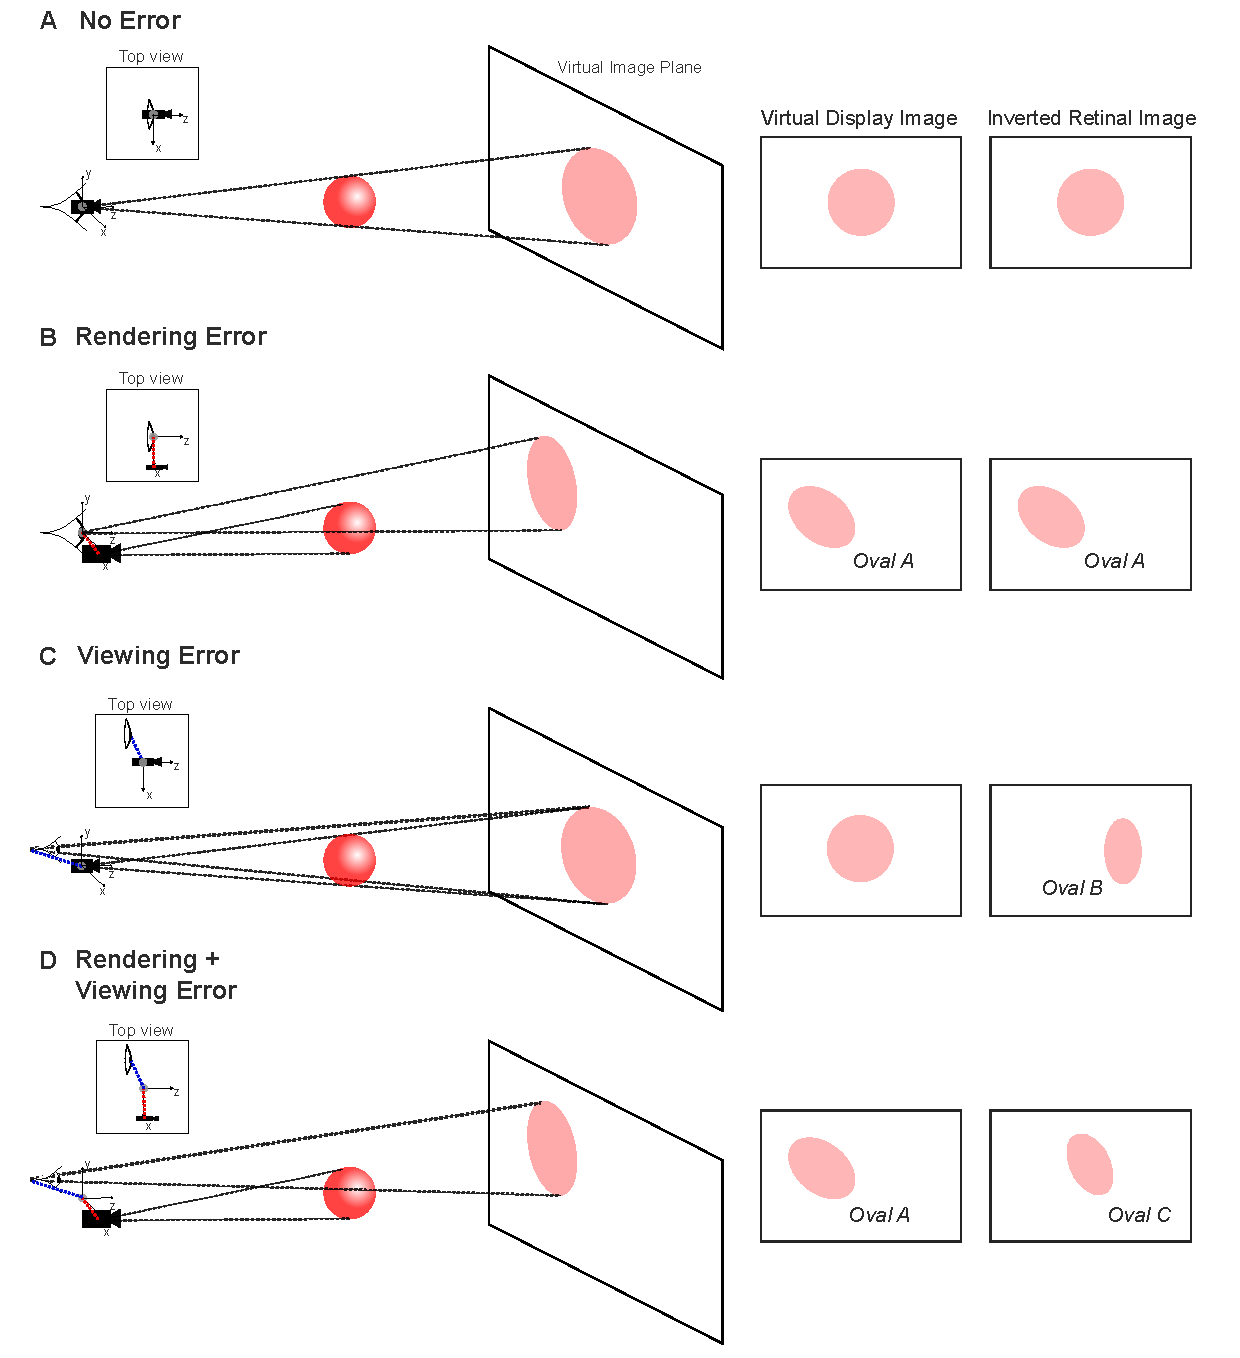
\includegraphics[width=\linewidth]{figures/model/rendering_vs_viewing_error.pdf}  
	     \caption{Comparing rendering error with viewing error. For simplicity, we show a monocular example as the set up is the same for both eyes. The origin of the coordinate system is at the HMD CoP (grey dot). The virtual sphere is positioned directly in front of the the HMD CoP. \textbf{(A)} In the ideal scenario, the render camera, CoP of the user's eye, and HMD CoP are all at the same position in space. No rendering or viewing error exists in this system. The camera is on-axis with the sphere and will render the corret perspective projection (a circle) that will be presented on virtual image plane. The user will view this circle from the intended CoP and the user's retinal image of what is shown on the display plane is also a circle. \textbf{(B)} The render camera is displaced to the right and down from the HMD CoP, creating a rendering error. The camera will render the sphere from this incorrect location, and render an oval instead of a circle. This oval is shown on the display plane and the user views it from the correct position so they perceive the same incorrectly rendered oval. \textbf{(C)} The CoP of the user's eye is displaced to the left and behind the HMD CoP, creating a viewing error. Despite the rendered image being correct on the virtual image plane, the perceived image is distorted. \textbf{(D)} In realistic usage, rendering and viewing errors typically occur together and can result in geometric errors being introduced in both render and viewing stages.}
	     \label{fig:rendering_vs_viewing_error}
	 \end{figure}


\subsection{Coordinate Systems and Distance Measurement}
Distance perception in HMDs involves two distinct coordinate systems. The origin of the \textit{HMD coordinate system} is centered between the two HMD CoPs; the intended virtual scene is defined within this frame. However, the user perceives distance relative to their own body. The \textit{egocentric coordinate system} is therefore defined relative to the viewer, with the origin centered between the user's actual left and right eye CoPs.

Ideally, these two systems align. However, viewing errors—such as eye relief shifts—introduce offsets between the egocentric and HMD frames (this is a simplified framework that does not account for the optical effects of HMD optics). This misalignment has critical implications for measuring distance perception. For example, consider a viewer with a $+3$~cm eye relief error fixating on a target at the virtual image distance (VID) (Figure~\ref{fig:error_choices}C). While the target's position is unchanged in the HMD frame, the user's eyes are physically closer to the VID. Consequently, the distance perceived in the egocentric frame is $3$~cm shorter than the distance defined in the HMD frame (Figure~\ref{fig:geometric_model}).

Crucially, standard blind reaching tasks tracked via external systems typically report positions in HMD coordinates, thereby missing this egocentric shift. To address this, Section~\ref{sec:reaching} leverages eye tracking to record reaching data that explicitly accounts for the offset between egocentric and HMD coordinates. This allows us to analyze data in either frame, distinguishing between reach accuracy (HMD frame) and accurately perceived distance (egocentric frame).


% Near-eye optics in an HMD generally have an eyebox, a volume of space from which the user should view the display for the acceptable image quality \cite{cholewiak2020}. Within the eyebox there is usually a nominally designed location where image quality is best. This location is typically selected as the display CoP typically positioned when the user's actual eye position is unknown~\cite{Rong25}. 


%In ideal circumstances an HMD will fit on a viewer's head exactly as designed and the HMD (i.e., world) coordinate frame will be exactly aligned with the user's egocentric reference frame. However, some viewing errors such as an eye relief error will shift the headset's coordinate system relative to user. When this occurs the distance perceived by the user will not directly map to the intended distance in the headset's coordinate frame. For example, consider a case where a viewer fixates on a point rendered on the optical display plane with a -3 cm eye relief error (i.e, the viewer's eyes are 3 cm farther away from the display than expected). Since the fixation target is on the display plane, the user will also perceive the point at the display plane. In HMD coordinates there is no error since the perceived point is at the intended location (i.e., on the display plane). However, in egocentric coordinates the perceived point will be 3 cm farther from the user than specified by the virtual geometry (Figure~\ref{fig:geometric_model}). 

% Consider moving these to the discussion
%The difference between perceived distance in egocentric and HMD coordinates is not simply a semantic distinction. If the viewer were perfectly accurate at estimating distance, then a verbal distance estimate would be 3 cm larger than the distance measured by an outside observer or tracking system. In other words, characterizing distance perception using verbal report and blind reaching could lead to different conclusions. In some cases, egocentric and HMD measurements can lead to opposite conclusions. In Figure~\ref{fig:geometric_model} the row of objects in front of the display closest to the viewer will appear to be too far away if measured using blind reaching, and too near if measured using verbal reports. Similarly, the middle row of objects at and near the display plane will be measured at the correct locations in HMD coordinates (i.e., with blind reaching), but will be recorded as too close in egocentric coordinates (i.e., verbal estimate). This a critical point that illustrates the importance of measuring errors using a clear, consistent framework. Notably, we can analyze reach data in both coordinate frames because we measure each participant's actual user eye position in our HMD with an eye tracker. This allows us to transform the data into the appropriate coordinate frame to evaluate absolute reach accuracy in HMD coordinates and perceived distance in egocentric coordinates.

% Here the intended target is rendered at 40 cm from the headset's original (i.e., world coordinates). If the user is asked to reach for the target object, they will reach farther than the intended target in the headset's coordinate frame. However, the user actually perceives the target object to be closer than 40 cm, and so perceived error could be categorized as either an overestimated or underestimated distance depending on the coordinate frame.

% \begin{figure}
%     \centering
%     % \includegraphics[width=1\linewidth]{figures/model/Untitled.png}
%     \includegraphics[width=1\linewidth]{figures/model/egocentric_frame.png}    
%     \caption{Placeholder.}
%     \label{fig:egocentric_frame}
% \end{figure}

% Since we show people images of the wrong thing from the right place, we don't get the same effect as if people saw the right thing from the wrong place. Need to do a simple transform to get things back into the expected world-centric cooridnate frame instead of egocentric.
% In the absence of viewing error, these two reference frames are the same, however, viewing errors always offset these two reference frames.

\subsection{HMD Error Simulation Platform} \label{sec:hmd_platform}
\paragraph{Hardware}
We integrated a 240 Hz Tobii (Tobii AB, Sweden) eye tracker into a Meta Quest 3 (v72). For each user, lens were physically adjusted to match the user's IPD. For reaching experiments in Section~\ref{sec:reaching}, we tracked controller 3D position using the default Quest API. We measured controller tracking accuracy and found that tracking is accurate within 1.5 mm error across ten distances from 5 to 50 cm, measured from the front surface of the headset (see supplementary materials). 

\paragraph{Software} 

%We build a rendering pipeline in Unity (v2022.3.30f1) that can simulate the rendering and viewing errors outlined in Section~\ref{sec:model overview}. Our application uses multiple cameras and quads for ray capture and reprojection to accomplish this, and a high-level overview is provided here. Step-by-step rendering details are provided in the supplementary materials. First a pair of render cameras render the scene and sends their framebuffers to a pair of quads simulating the virtual displays in front of HMD CoP. The VID (virtual image distance) was set to 1.3 m, approximating a reasonable VID similar to most modern HMDs designed minimize vergence-accommodation conflict~\cite{hoffman2008vergence}. Render error can be applied as a displacement of the render camera from the HMD CoP. Next, a pair of "viewing" cameras (implemented as standard camera object) view the virtual display quads from the previous step. The viewing cameras are meant to simulate user CoP in our \textit{simulated} headset space. Viewing error is applied as a displacement of the viewing camera from the HMD CoP. Lastly, the user's eyes are unlikely to be at the nominally assumed position within the Quest 3 eyebox, so we must also compensate for this naturally-occurring viewing error in the headset. This is accomplished by placing a pair of quads showing viewing camera's framebuffer in front of the actual user's 3D pupil positions from the eye tracker. These quads showing the user's expected view of the simulated rendering and/or viewing errors are imaged by the standard OVRCameras (which are positioned at actual headset CoP, not at the user's actual eye position) and this framebuffer is shown on the Quest 3 display. 

We build a rendering pipeline in Unity (v2022.3.30f1) that can simulate the rendering and viewing errors outlined in Section~\ref{sec:model overview}. The simulated headset origin is set to the midpoint of simulated HMD CoPs, positioned at (-$\frac{IAD}{2}$, 0, 0) and ($\frac{IAD}{2}$, 0, 0) for the left and right eyes, where IAD is the interaxial distance of the simulated headset. For simplicity, we first describe the rendering algorithm for one eye only (right eye). In the rendering stage, the rendering error is the displacement $\mathbf{{E}_{rendering}}$ of the rendering camera from the HMD CoP. For an arbitrary point in the scene $\mathbf{P}$, the ray vector captured by the rendering camera is: 

\begin{equation}
	\mathbf{C} = \mathbf{P} - \mathbf{{E}_{rendering}} - (\frac{IAD}{2}, 0, 0)
\end{equation}

The captured ray is then projected onto a quad positioned at the VID (virtual image distance). The VID is set to 1.3 m, approximating a reasonable VID similar to most modern HMDs designed minimize vergence-accommodation conflict~\cite{hoffman2008vergence}. The line of projection is: 

\begin{equation}
	\label{eqn: rendering_line}
	\mathbf{R} =m \mathbf{C} + (\frac{IAD}{2}, 0, 0),  m \in \mathbb{R}
\end{equation}

The projected point is intersection of the ray with the quad and found by setting $R_{y}=VID$ and solving for $m_{0}$. Substitute $m_0$ into Equation \ref{eqn: rendering_line} gives $\mathbf{R_{0}}$. This completes the rendering stage. 

For the viewing stage, the simulated eye is displaced from the HMD CoP by the viewing error vector $\mathbf{E_{viewing}}$ and views the projected point $\mathbf{R_{0}}$. The viewing ray is: 

\begin{equation}
	\mathbf{V} = \mathbf{R_{0}} - \mathbf{E_{viewing}}- (\frac{IAD}{2}, 0, 0)
\end{equation}

Lastly, we present the simulated view to the user's actual eye. The user's eye is unlikely to be at the nominally assumed position within the Quest 3 eyebox, so we must compensate for this naturally-occurring viewing error. This is accomplished by tracking the 3D pupil position using the eye tracker and presenting the simulated view on a quad based on the actual eye position. The actual HMD origin is the midpoint of Quest 3 CoPs positioned at ($-\frac{IPD}{2}$, 0, 0) and ($\frac{IPD}{2}$, 0, 0) for the left and right eyes. The tracked eye position is \textbf{E} and the line of projection is: 

\begin{equation}
	\label{eqn: rendering_line_from_actual_eye}
	\mathbf{R'} = \mathbf{E} + n \mathbf{V},   n \in \mathbb{R}
\end{equation}

The projected point is again found by setting $R'_{y}=d$, where $d$ is the fixed distance of the quad from the actual eye and solving for $n_{0}$. Substituting $n_{0}$ into Equation \ref{eqn: rendering_line_from_actual_eye} gives the intersection point $\mathbf{R'_{0}}$. The standard OVR camera positioned at the Quest 3 CoP then views the projected point $\mathbf{R'_{0}}$ and the ray is: 

\begin{equation}
	\mathbf{V'} = \mathbf{R'_{0}} - (\frac{IPD}{2}, 0, 0)
\end{equation}

The rendering algorithm for the left eye is the same as the right eye except $\frac{IAD}{2}$ and $\frac{IPD}{2}$ are replaced with $-\frac{IAD}{2}$ and $-\frac{IPD}{2}$. The percieved point in actual HMD coordinate system ${\textbf{P}}^{HMD}_{perceived}$ is given by the intersection of the left and right rays, which is found by setting them equal to each other:

\begin{equation}
	h \mathbf{V'_{left}} - (\frac{IPD}{2}, 0, 0) =l \mathbf{V'_{right}} + (\frac{IPD}{2}, 0, 0), h, l \in \mathbb{R}
\end{equation}

The solutions are: 

\begin{equation}
		l = \frac{IPD \sqrt{{v'_{left_{y}}}^2+{v'_{left_{z}}}^2}}{\vert \mathbf{V'_{left}} \times \mathbf{V'_{right}}\vert} , h = \frac{IPD \sqrt{{v'_{right_{y}}}^2+{v'_{right_{z}}}^2}}{\vert \mathbf{V'_{left}} \times \mathbf{V'_{right}}\vert} 
\end{equation}

The perceived point in egocentric coordinate system is obtained by subtracting off the translation of the interocular axis origin from the HMD origin: 

\begin{equation}
	{\textbf{P}}^{egocentric}_{perceived} = {\textbf{P}}^{HMD}_{perceived} - (0, 0, E_{eye\,relief})
\end{equation}

The experimentally measured natural eye relief error $E_{eye\,relief}$ was 13 mm on average (Table 1, supplementary materials). More information on the rendering pipeline can be found in the supplementary materials where we provide step-by-step ray tracing diagrams for illustration.

% For this we estimate actual user CoP by querying their 3D pupil positions from the eye tracker and present the frame buffers of the viewing cameras in front of the actual user CoP via another pair of quads.


%First, we estimate user CoP by querying their 3D pupil position from the eye tracker and determine the offset from the HMD CoP. This offset is applied to the OVRCamera object in Unity and is the position used for left and right HMD CoPs in Figure~\ref{fig:teaser} A. Render cameras Quads representing the left and right eye virtual displays are positioned at the VID in front of each of the HMD CoPs. Rendering error is applied as a displacement to a camera relative to the HMD CoP, and the framebuffer from the render camera is drawn to the virtual display quad. Viewing error is applied as a relative displacement between the HMD CoP and a viewing camera which images the display quad. Finally, the framebuffer from the left and right eye viewing cameras are viewed by the OVRCameras and projected onto the real HMD displays.

%\paragraph{Coordinate Frames} In our system we track user eye position and compensate for any naturally occurring viewing errors due to variations in headset fit. We then simulate and show users what they would have seen if their eyes were in a location that can be arbitrarily specified (e.g., with rendering or viewing errors). Consequently, we can show all participants the same simulated errors, regardless of where their eyes actually are. However, this means that interpreting reaching measurements from our HMD simulation platform is not always directly comparable to reach distance obtained in a headset with the actual errors being simulated.

%There are two important coordinate frames in our study: (1) HMD coordinates, and (2) egocentric coordinates. All reach data is recorded in HMD coordinates, but blind reaching data cannot be directly interpreted using these values. Since blind reaching is an open-loop task, reach distances are made in egocentric coordinates (i.e., a distance relative to the participant) so any offsets between egocentric and HMD origins must be accounted for (e.g., any eye relief errors that offset the HMD origin from the viewer's cyclopean eye). Therefore blind reach distances presented in HMD coordinates are first converted into egocentric coordinates, then converted back into HMD coordinates based on the simulated viewpoint position, rather than actual viewer position. The second transform from the viewer's actual eye position to the simulated viewpoint is important to illustrate where a participant would reach if their eyes were at the simulated location, rather than where their eyes actually are. Sighted reaching is a closed-loop task so participants must reach to the actual intended distance in HMD coordinates to generate the same stereo geometry as shown in the target interval, and egocentric conversions are unnecessary for sighted reaches. More details are provided in the supplementary materials. 
	\section{How Accurately Does Geometry Predict Blind Reach Distance?} \label{sec:reaching}
To understand how stereo geometry errors in HMDs affect near-field distance perception, and specifically how changes in perceived distance impact reaching behavior, we compared participants' blind reaching errors against the stereo triangulation model described in in Section~\ref{sec:model overview}.

% To understand how stereoscopic geometric errors in HMDs affect distance perception in the near field, we performed a series of blind experiments in an HMD with different rendering and viewing errors. We compared participants' blind reaching errors to the predictions of our simple triangulation model in Section \ref{sec:model overview} to test how well misperceptions of distance in HMDs can explained by errors in stereo geometry alone. 

\subsection{Error Condition Selection} \label{sec:exp1_procedure}
We evaluated three rendering and viewing errors critical to current VR hardware designs (Figure~\ref{fig:error_choices}).

% We measured blind reaching in a real world task to establish a per-subject comparative baseline for in-HMD blind reaching performance and describe the methods to measure each below.
% We ran a series of experiments to examine the conditions outlined in Section~\ref{sec:conditions} and real life blind reaching experiment to establish a comparaitive baseline for our VR reaching tasks.

\paragraph{Direct Passthrough Rendering Error}
Video passthrough headsets can use view reprojection \cite{ElChemalyGAP, xiao2022neuralpassthrough} or computational imaging \cite{kuo23} to correct for the positional offset between the passthrough cameras and the viewer's eyes. Alternatively, "direct passthrough" avoids these computationally expensive methods, and potential image distortions associated with them, by directly streaming perspective-incorrect video. To simulate this effect, we displaced the render cameras by 5.5 cm—a value representative of the thickness of current commercial headsets. We also simulated a -5.5 cm error for completeness (Figure~\ref{fig:error_choices}A).

\paragraph{IPD Viewing Error}
Perceived depth is inherently tied to retinal binocular disparity and a user's IPD. Failure to match the headset's interaxial distance (IAD) to the user's IPD creates a viewing error (not a rendering error because the render cameras and HMD CoP are colocated) and the user will experience incorrect disparity and vergence demand at the fixation point. We picked 12 mm errors based on a worst-case error in real life HMD use (Figure~\ref{fig:error_choices}B).

\paragraph{Eye Relief Viewing Error}
Due to differences in facial geometry, a viewer's actual nominal eye position in the headset may be displaced from this assumed location. We picked 3 cm as a potential eye relief viewing error which represents a value that is as large as could be reasonably expected for a typical HMD optical design (Figure~\ref{fig:error_choices}C).

\subsection{Participants}
Thirty-two participants (mean age: 32.2 years, $\sigma=7.2$; mean IPD: 62.7 mm, $\sigma=2.6$) with normal or corrected-to-normal visual acuity of 20/20 and Randot stereo acuity <= 50 arc seconds participated in the study. All study protocols were IRB approved.

\subsection{Methods}
\paragraph{Real Life Blind Reaching}
To check for inherent reaching biases, participants viewed a physical coin at 30 cm, closed their eyes, and reached for it. During the task, each participant's head was stabilized in a chin rest. A coin was placed on the table at 30 cm away from their forehead by the experimenter and participants were asked to remember its position. They then closed their eyes, after which the coin was removed by the experimenter, and were asked to reach for the coin's location. Participant's eyes remained closed until reach distance was recorded and their arm was back at their side. The participant was not made aware that the coin was placed at the same distance on each trial. This process was repeated three times to assess baseline blind reaching performance in real life.

\paragraph{In Headset Blind Reaching} 
Participants viewed a virtual controller at 30 cm (Figure~\ref{fig:teaser}E), hid the controller via a button press, and reached for the remembered location with a real controller. They had unlimited time to view the virtual controller and pressed a button on the left controller to hide the target when they were ready to start their reach with the right controller. Once they were satisfied with their controller placement, participants pressed another button on the left controller to record the right controller's position, and returned their right hand with the controller to a comfortable resting position. There were seven conditions in total: $\pm$ 55 mm direct passthrough rendering error, $\pm$ 12 mm IPD viewing error, $\pm$ 30 mm eye relief error, and a no error condition. The testing order of conditions was random and participants completed a total of 210 trials (30 trials for each condition) in a single session. Participants were asked to minimize head movement. An outlier analysis was performed for each condition to remove trials that appeared to be inadvertent completions where at least one of three coordinates of the controller was recorded beyond lower or upper fences (1st quartile - 1.5 times the interquartile range (IQR) or 3rd quartile + 1.5 IQR) of the recorded reach positions. On average this led to the removal of 2 trails ($\sigma$ = 1.7) per condition (30 trials).


\paragraph{Data Transforms}
Two transforms were applied to the reaching data. First we apply bias correction to account for each participant's baseline blind-reaching bias from the real-life reach (Figure~\ref{fig:bias_plot}, right marker). These transformed values are shown in Figure~\ref{fig:reaching_HMD_coordinates} (right marker of each panel). For the second transform, we converted distances from HMD coordinates to egocentric coordinates (Section \ref{sec:model overview}) since perceived distance by definition is in an egocentric coordinate frame. The transformed egocentric distance values are shown in Figure~\ref{fig:reaching_egocentric_coordinates}. This second transform only affects values in the eye relief error condition as HMD coordinate frame and egocentric coordinate frame are offset by 3 cm (Figure \ref{fig:error_choices}C). 

\subsection{Statistics}
Linear mixed effects models (LMEM) were used to estimate the influence of rendering and viewing errors on the magnitudes of reaching errors. In all cases, we specified a maximal model by default (i.e., including random intercepts and slopes for all relevant factors) following \cite{Barr2013RandomES,Harrison2018ABI, MixedEffectsLME4, maxwell2017StatsBooks}. For the reaching data, the maximal model was

\begin{equation}
\begin{split}
    \text{reachBias} \sim \text{error}
    + \space (\text{error} \mid \text{ID})
\end{split}
\end{equation}

where error was the magnitude in centimeters of the rendering or viewing error — for example, for direct passthrough: -5.5, 0, or 5.5 cm; reachBias was the bias of the average reach endpoint in egocentric coordinates, after also subtracting off any biases observed in the 0 cm / no-error condition. ID was simply each participant ID. 

\begin{figure}
	\centering
	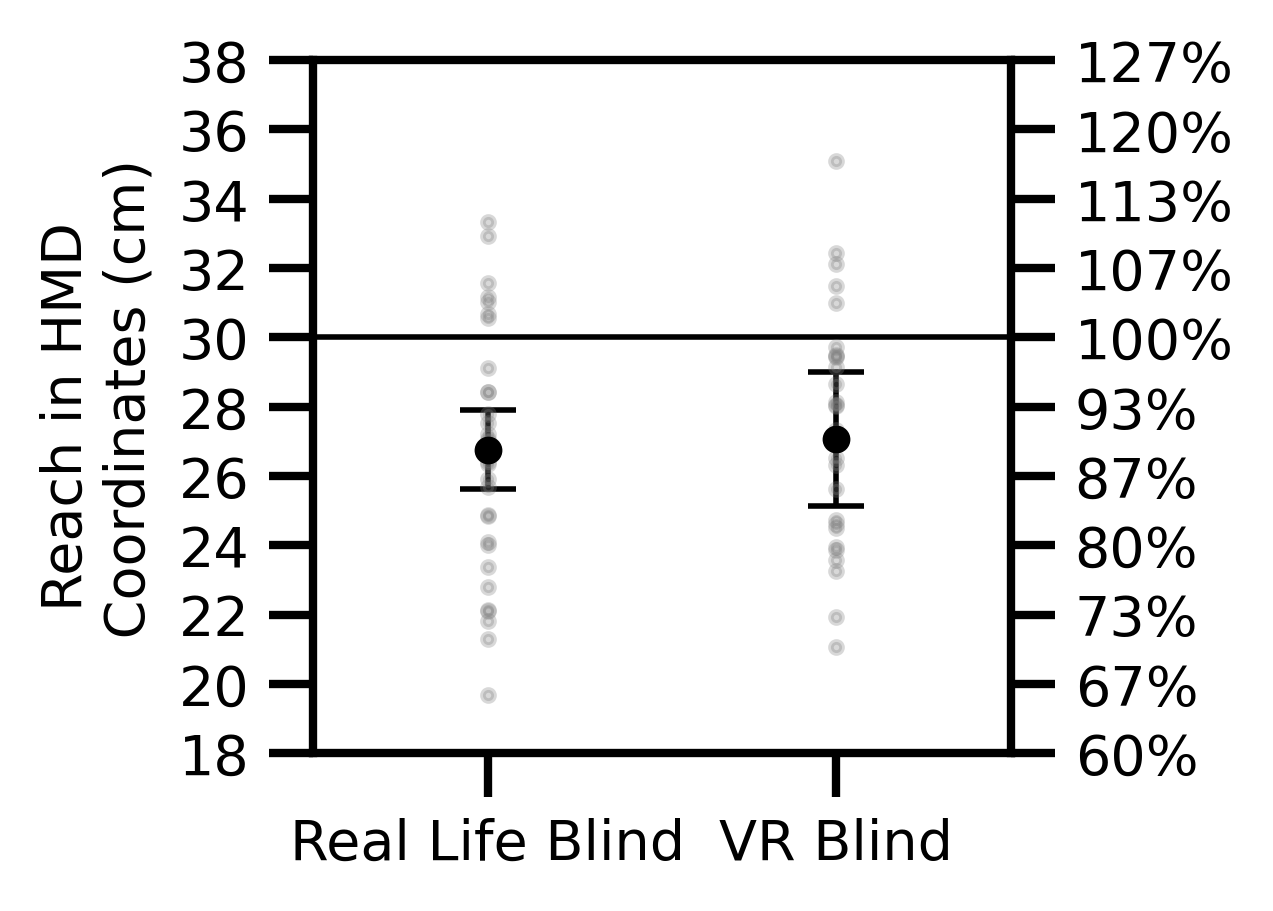
\includegraphics[width=0.65\linewidth]{figures/reaching/real_life_VR_reaching_comparison.png}
	\caption{Blind reaching with correct stereo geometry (no viewing or rendering errors). Black points show the average reach distance and 95\% confidence intervals across all participants (n=32) for a target positioned 30 cm away in HMD coordinate system. Grey points show individual participant data. On average, participants under-reach in both real-life and VR blind reaching conditions by approximately 10\%. 
	}
	\label{fig:bias_plot}
\end{figure}


\begin{figure}[]
    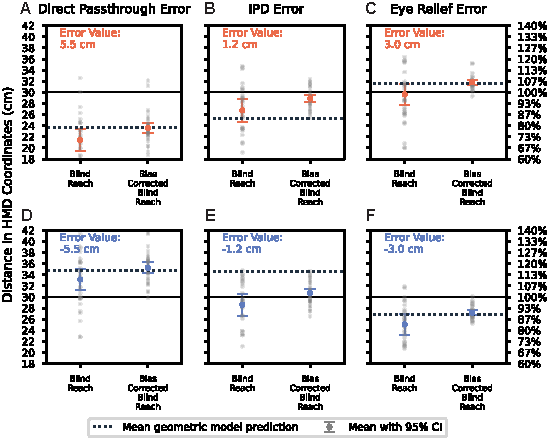
\includegraphics[width=\linewidth]{figures/reaching/reaching_HMD_coordinates.pdf}
    \caption{Reach distance in HMD coordinates for blind reaching and blind reaching corrected for under-reaching bias for \textbf{(A)} direct passthrough error, \textbf{(B)} IPD error, and \textbf{(C)} eye relief error. Positive errors are shown in the top row (red) and negative errors are shown in the bottom row (blue). Black points are means with error bars denoting 95\% confidence interval (n=32). After accounting for participant under-reaching bias, blind reach distances are well-predicted by our model for direct passthrough error and eye relief error.}
    \label{fig:reaching_HMD_coordinates}
\end{figure}

\subsection{Results}
\label{sec:exp1results}
Geometric errors induced statistically significant changes in perceived distance across all conditions. Notably, the magnitude of these shifts aligned closely with geometric predictions for direct passthrough and eye relief errors. In contrast, the observed effect of IPD error, while significant, was substantially smaller than the geometric model predicted.

\paragraph{No Rendering or Viewing Error}
Participants consistently under-reached the $30$~cm target (hypometric reaching) in both VR and real-world baselines (Figure~\ref{fig:bias_plot}). Across 32 participants, endpoints fell short by approximately $3$--$4$~cm ($\sim10\%$). The difference between real-world and VR performance was not statistically significant (paired t-test: $t = 0.71, p = 0.47, df = 31$), suggesting that the under-reaching observed in this study shares a common etiological origin with natural proprioceptive or visual biases rather than being an artifact of the VR hardware.

\paragraph{Direct Passthrough Error}
Participants underestimated distance when the render cameras were offset forward (Figure~\ref{fig:reaching_egocentric_coordinates}A). The LMEM revealed a near-perfect linear relationship between the physical offset and the perceptual error ($\beta = -1.07, t = -13.87, p < 0.0001$). This slope indicates a $\sim1$~cm underestimation of distance for every $1$~cm of forward camera displacement. These results confirm that distance misperception caused by direct passthrough offsets is well-described by simple triangulation geometry.

\paragraph{IPD Error}
Perceived distance scaled inversely with IPD error (Figure~\ref{fig:reaching_egocentric_coordinates}B). When the HMD IAD exceeded the user's IPD, targets appeared closer ($\beta = -0.76, t = -3.20, p < 0.02$). This implies a $0.76$~cm underestimation for every $1$~cm of excess IAD. While the effect is significant, the geometric model over-predicts the magnitude of this error, suggesting that the visual system may partially compensate for IPD mismatches (discussed further in Section~\ref{sec:discussion}).


\begin{figure}
	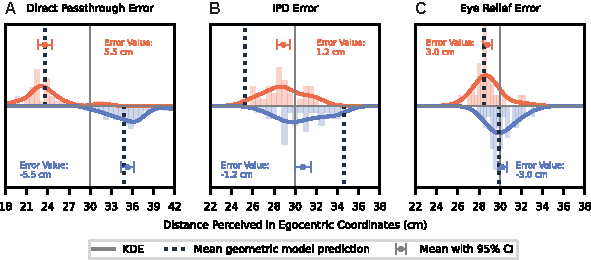
\includegraphics[width=\linewidth]{figures/reaching/egocentric_distance_summary.pdf}
	\caption{Perceived distance in egocentric coordinates induced by rendering and viewing errors compared to model predictions. Each participant's blind reaching performance is adjusted to account for their no-error blind reach baseline for \textbf{(A)} direct passthrough error, \textbf{(B)} IPD error, and \textbf{(C)} eye relief error. For each, the red histogram shows individual data (n=32) for positive error while the yellow histogram is for negative error. A kernel density estimate (KDE) is shown to visualize the distribution. \textbf{(A)} and \textbf{(B)} replot data from Figure \ref{fig:reaching_HMD_coordinates}A-B (right most data points) since HMD coordinate system overlaps with egocentric coordinate system for those two error types. Our model predictions in egocentric coordinates provide good account of the data for direct passthrough error and eye relief error, but not for IPD error. A statistically significant effect is found in all three conditions when using a general linear mixed model to examine the relationship between error magnitudes and reach accuracy.}
	\label{fig:reaching_egocentric_coordinates}
\end{figure}


\paragraph{Eye Relief Error}
Eye relief errors produced a significant linear shift in perceived distance ($\beta = -0.23, t = -5.38, p < 0.0001$). A $+3$~cm error (eyes closer to display) caused the target to appear closer than intended. Conversely, a $-3$~cm error (eyes further from display) resulted in reaches that appeared accurate in the egocentric frame (Figure~\ref{fig:reaching_egocentric_coordinates}C). 

This apparent accuracy is due to a cancellation effect at this specific target distance: the \textit{optical error} (which geometrically pushes the virtual image away) is effectively neutralized by the \textit{egocentric frame shift} (the user standing $3$~cm further back). Although these factors canceled out at $30$~cm, the linear model confirms that our geometric predictions accurately account for the underlying trend in both positive and negative directions.
	\section{How much stereo geometry error is detectable?} \label{sec:visual}
While direct passthrough errors elicited a reaching response consistent with geometric predictions, the impact of IPD errors was significantly weaker than predicted. This suggests that the visual system may be robust to—or perhaps less sensitive to—IPD mismatches compared to rendering offsets. To determine if this reduced behavioral sensitivity corresponds to a higher perceptual detection threshold, we conducted a follow-up psychophysical experiment using a two-interval forced choice (2IFC) task.

% We found in Section~\ref{sec:exp1results} that the magnitude of misperception induced by IPD error is much smaller than predictions of the geometric model. This result shows the underlying mechanism for distance judgment is only weakly sensitive to stereo cues in the IPD error condition. We wondered if this would also make IPD error be less detectable than what stereo geometry predicts. The next set of experiments directly measured detection thresholds for IPD error and direct passthrough error using a two interval forced choice (2IFC) task. 

%In the strictest sense, the distance that someone blind reaches is not a direct measure of perceived distance. We have shown in the previous section it is subject to a level of baseline bias, when corrected, aligns with our geometric model for two of three error conditions but not IPD error. In this next set of experiments we directly measured the perceived visual distance of an object using a psychophysical paradigm to directly interrogate the effects of errors in stereo geometry on distance perception. We used a two-interval forced choice (2IFC) task to determine whether an object with a purposefully induced rendering or viewing error appeared closer or farther than the same object rendered and viewed with accurate stereo geometry -- a task that is only possible in a platform like the the one described in Section~\ref{sec:hmd_platform}. Each instance of this judgment was fast, which allowed us to accumulate enough trials to extract the detection threshold from the psychometric function. These error detection thresholds were used to test the efficacy of our geometric model.

%The underlying visuomotor mapping from vision to reaching is also a process that is plastic and adaptable \cite{krakauer2000learning}.

\subsection{Participants}
The same 32 participants that performed the reaching experiments participated in this study and all protocols were IRB approved.

\subsection{Methods}
In each trial, participants viewed a red sphere in two successive intervals: a reference interval (rendered with correct stereo geometry) and a comparison interval (rendered with either a direct passthrough or IPD error). The interval order was randomized, and each interval lasted 800 ms with a 200 ms inter-stimulus interval. Participants indicated which interval appeared closer via controller input. The monocular size of the sphere in the reference interval was always fixed at 1$^\circ$, but scaled naturally according to perspective geometry in the comparison interval. We used the Method of Constant Stimuli to sample the psychometric function, varying error magnitudes in 100 equal steps ($\pm 12$~mm for IPD; $\pm 100$~mm for direct passthrough). Each participant completed 1200 trials (2 error types $\times$ 3 distances $\times$ 2 scenes $\times$ 100 repetitions) in randomized order, separated into three blocks for each viewing distance.



\begin{figure}
	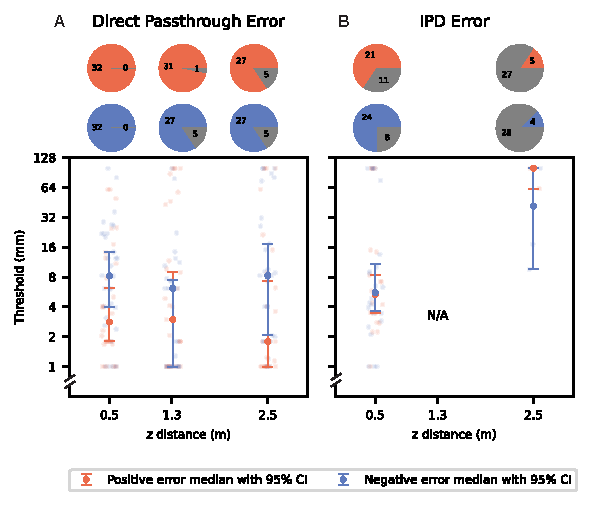
\includegraphics[width=\linewidth]{figures/visual/detection_thresholds_with_background.pdf}
	\caption{Detection thresholds for \textbf{(A)} direct passthrough error and \textbf{(B)} IPD error. Red and blue points are detection thresholds for positive and negative error directions. For IPD error, a positive error means HMD IAD is larger than user IPD and vice versa. For direct passthrough error, a positive error means rendering cameras are in front of HMD CoP and vice versa. Pie chart shows split of participants that were sensitive to the specific error type (red or blue) and sign vs those who performed at chance (gray). For target placed 1.3~m and affected by IPD error, our geometric model predicts no error and detection threshold is ill-defined.}
	\label{fig:detection_thresholds_with_background}
\end{figure}

\subsection{Viewing Conditions}
We expected sensitivity for both error types to depend on viewing distance and scene content. We varied distance and visual scene to explore the effects of three specific perceptual phenomenon.

% \begin{itemize}
    \paragraph{Stereo Sensitivity Gradient (IPD)} Binocular disparity cues degrade non-linearly with distance ($1/d^2$) \cite{howard2012perceiving}. We selected test distances of $0.5$~m (Near), $1.3$~m (Intermediate/VID), and $2.5$~m (Far). We hypothesized that IPD errors, which rely on disparity and vergence shifts, would be more detectable in the near field, undetectable at the VID (because viewing errors do not introduce geometric errors at the VID), and less detectable $2.5$~m.
    \paragraph{Weber's Law (Passthrough)} For direct passthrough, the rendering error represents a depth offset ($\Delta d$). According to Weber's Law, the Just Noticeable Difference (JND) should scale with total distance ($\Delta d / d = k$). Therefore, we expected thresholds to be lowest at $0.5$~m and highest at $2.5$~m.
    \paragraph{Cue Integration (Scene Content)} We utilized two environments to modulate cue reliability. A complex scene provided strong monocular cues (linear perspective, height-in-field) that may conflict with or override erroneous stereo cues. A sparse scene showed only a fixation target with a Skybox background, and this reduced scene may increase sensitivity to IPD errors compared to the structured environment.
% \end{itemize}

\subsection{Psychometric Function Fitting}
% \paragraph{Psychometric Function Fitting}
We excluded participants who were not sensitive enough to the combination of error type and error sign by performing a one-tailed binomial test (alpha value 0.05), which determines whether psychometric performance is different from chance (50\%). We estimated detection thresholds by fitting a psychometric function to the log-transformed error values for positive and negative errors separately. Additional details are provided in Supplementary Materials. 

% \paragraph{Linear Mixed Effect Modeling}
% Like the reaching experiments we specified another linear mixed effects model (LMEM) to evaluate the impact of error type, viewing distance, and background on each participant's detection threshold. The maximal model in for this analysis is:
% \begin{equation}
%     \text{threshold} \sim \text{distance} * \text{scene} + (\text{distance} * \text{scene} \mid \text{ID})
% \end{equation}
% where detection threshold was the best-fit threshold of a single participant's psychometric function. We used the beta coefficients and associated p-values for the fixed effect slope and intercept terms of interest to make statistical decisions.

\begin{figure}
	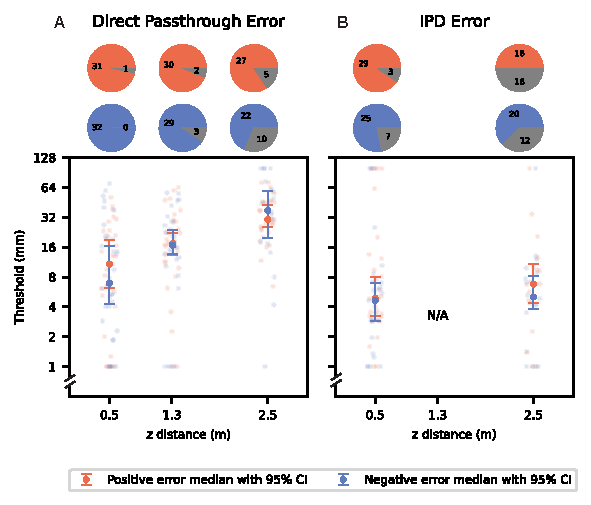
\includegraphics[width=\linewidth]{figures/visual/detection_thresholds_no_background.pdf}
	\caption{Detection thresholds for \textbf{(A)} direct passthrough error and \textbf{(B)} IPD error with only the skybox scene.
	}
	\label{fig:detection_thresholds_no_background}
\end{figure}


\subsection{Results} \label{sec:exp2results}
\paragraph{Error Detectability in Naturalistic Conditions}
We first assessed the absolute range of perceptible errors in the naturalistic environment (the Forest scene).  Overall we identify trends that are consistent with our expectations, IPD error is perceptible at near distances and nearly imperceptible at far distances (Figure~\ref{fig:detection_thresholds_with_background}B).  However, participants have a surprisingly high threshold for IPD errors, at approximately 6 mm. This relatively large error required for detection (approximately 10\%) is consistent with our reaching results, which show that IPD errors have a smaller than expected impact on reach distance. At intermediate ($1.3$~m) and far ($2.5$~m) distances, psychometric functions were predominantly flat, indicating that most participants could not distinguish the error from the reference. Additionally, at the VID, the geometric model predicts zero geometric distortion for viewing errors; consequently, an objective ground truth for "correct" interval identification—which is required to extract detection thresholds—is theoretically undefined.

To confirm whether participants were performing above chance, we applied a one-tailed binomial test to the psychometric fits. The results confirmed widespread insensitivity to IPD mismatches. Out of 64 fits at the far and intermediate distances, only 7 exhibited performance significantly above chance at the far distance resulting in an IPD detection threshold of $>$41 mm. Insensitivity persisted for some even at $0.5$~m, where stereo cues are strongest; 13 participants failed to exceed chance performance in at least the positive or negative IPD error conditions.

In contrast, participants were consistently sensitive to direct passthrough errors (Figure~\ref{fig:detection_thresholds_with_background}A). Median thresholds were between $1.8$--$3.0$~mm across viewing distances for positive errors, and $6.1$-$8.3$ for negative errors. Ulike IPD errors, the failure rate was minimal (only 16 failures total across all conditions), indicating a much more robust perceptual signal.

\paragraph{Scene Complexity}
In the naturalistic forest scene, depth cues other than stereopsis provide reliable distance information. In our sparse scene, where these other cues are removed, we observed that sensitivity to IPD errors improved dramatically, whereas sensitivity to direct passthrough errors decreased. Most notably, IPD viewing errors at the far distance were largely undetectable in the natural scene (55 of 64 psychometric functions), but detection rates improved significantly in the sparse scene (dropping to 28 of 64 undetectable cases). For participants who met the inclusion criteria in the sparse condition, median IPD error thresholds were 5.0 mm (negative) and 6.8 mm (positive) - a massive improvement from the 41.4 (negative) and 100 (negative) mm thresholds obtained from the 9 thresholds that met the inclusion criteria in the complex scene. At the near distance median IPD thresholds improved from 5.6 mm and 5.4 mm (natural) to 4.6 mm and 4.9 mm (sparse) for negative and positive errors, respectively. These results indicate that perceptual sensitivity to IPD errors is strongly dependent on scene content and increases when other depth cues are eliminated.

Conversely, sensitivity to direct passthrough rendering errors followed the opposite trend: median thresholds were substantially elevated (indicating lower sensitivity) across most conditions in the sparse scene. This is expected because the geometric impact of passthrough error diminishes as viewing distance increases. In the naturalistic scene, there are still objects located close to the viewer remain even when the target object is farther away, providing high-sensitivity references. The removal of these foreground objects in the sparse scene resulted in an approximately $3\times$ increase in thresholds at the far distance compared to the near distance.



% Participants' thresholds for direct passthrough error were higher overall in the skybox scene, and increased more rapidly as a function of viewing distance (1.13 mm vs. 0.355 mm per 1 m object distance; t = 3.06; p = 0.002 for the interaction of background presence and object distance). For IPD error, the opposite was observed (0.24 mm vs. 0.82 mm per 1 m object distance; t = -2.11; p = 0.036 on the same interaction). 
   
	\section{Discussion}
\label{sec:discussion}


\paragraph{Headset Optics}
Our study purposefully ignores the impacts of near-eye optics and treats the display stack as an idealized, perfectly head-locked planar display at a fixed VID. This is necessary abstraction in order to generalize our findings to all HMDs, but ignores the realities of real HMD optics. Our simplification treats viewing errors as purely as geometric translations of the view frustum, and this approach isolates the impact of geometric perspective errors while purposefully excluding optical effects. Real viewing errors with near-eye optics are a more complex interaction between the actual displacement from the nominal eye position and the optical design which introduces pupil swim and other optical aberrations. It is important to account for these differences when considering the impacts of viewing errors in real devices.

\paragraph{Implications for IPD Adjustment} Our results indicate that reach behavior remains robust even in the presence of significant IPD errors ($\pm$12 mm). We found that IPD offsets are generally imperceptible except at large magnitudes and close viewing distances (6 mm at 50 mm viewing distance). This aligns with prior research demonstrating a general insensitivity to absolute IPD mismatches in stereoscopic content \cite{allison2015perceptual, didyk2011, guan2016, stevenson1989hyperacuity}. While IPD shifts are known to alter the perceived scale of objects \cite{kim_dwarf_2017, piumsomboon_superman_2018, mine_relationship_2020}, their specific contribution to distance judgment remains unclear. However, perceptual tolerance does not eliminate the need for mechanical IPD adjustment. Physical IPD and IAD alignment is still required to mitigate view-dependent optical artifacts (such as blur and distortion), even if the user is geometrically insensitive to the perspective shift.

\paragraph{Implications for Video Passthrough}
While current commercial HMDs typically rely on static rendering pipelines, our results suggest that the geometric viewing errors inherent to these systems can induce perceptual inaccuracies. This is particularly critical for video passthrough HMDs. Unlike standard VR, where the virtual camera can be placed anywhere, passthrough cameras are physically constrained by the displacement between the external cameras and the user's eyes. Our findings support the adoption of computational imaging methods \cite{kuo23} or view-synthesis algorithms to correct this parallax mismatch \cite{ElChemalyGAP, xiao2022neuralpassthrough}. However, implementation requires a careful trade-off: the latency and potential image artifacts introduced by these methods can sometimes generate registration errors more severe than the original static offset. Consequently, alternative hardware approaches—such as reducing the physical camera-to-eye distance via thinner optics \cite{maimone2020holographic}—may act as a necessary complement to software correction to ensure perceptual accuracy.

\paragraph{Active vs. Static Observers}
Our study focuses on static observation to isolate specific geometric variables; however, real-world HMD usage involves continuous head and eye movement. Perspective projection errors that are imperceptible to a static observer often manifest as dynamic distortions—such as world instability or "swimming"—when the user moves \cite{guan2023perceptual}. These artifacts arise from discrepancies in motion parallax, a depth cue that can supersede stereoscopic cues in sensitivity. Consequently, the detection thresholds reported here may decrease with certain head and eye movements. Future work should extend this protocol to active observers to quantify the true limit at which geometric errors disrupt the stability of the virtual environment.


\section{Conclusion}
We highlighted the perceptual consequences of rendering and viewing errors in HMDs  To do this we first introduced a framework that differentiates between errors in stereo geometry introduced during rendering and viewing stages which can be clearly visualized in an accompanying interactive web application. We next built a software platform that corrects for naturally occurring and unavoidable viewing errors in a Quest 3 HMD which can then be used to purposefully simulate rendering and viewing errors. This platform enabled the set of blind reaching and two-interval forced choice experiments investigating the perceptual consequences of three ecologically-valid rendering and viewing errors in HMDs - a set of experiments that had not been previously possible despite their direct relevance to all egocentric, head-tracked display architectures.

We showed that errors in stereo geometry can induce changes in blind reach behavior but these blind reach distances need to be transformed to correct for reaching bias and put in the egocentric coordinate frame to be interpreted as perceived distance. Distance misperceptions induced by direct passthrough and eye relief errors are well predicted by our geometric model, but depth error induced by IPD error is smaller than predicted by geometry. Evaluating the detectability of IPD error in a 2IFC task revealed that, for a naturalistic and cue-rich scene, even detection thresholds for IPD errors was relatively high at 50 cm, and imperceptible to most viewers at 2.5 m. Overall, our findings demonstrate the perceptual impact of rendering and viewing errors in VR.
	\bibliographystyle{ACM-Reference-Format}
	\bibliography{bib}
        \nopagebreak 
        \begin{figure*}[h]
	\centering
	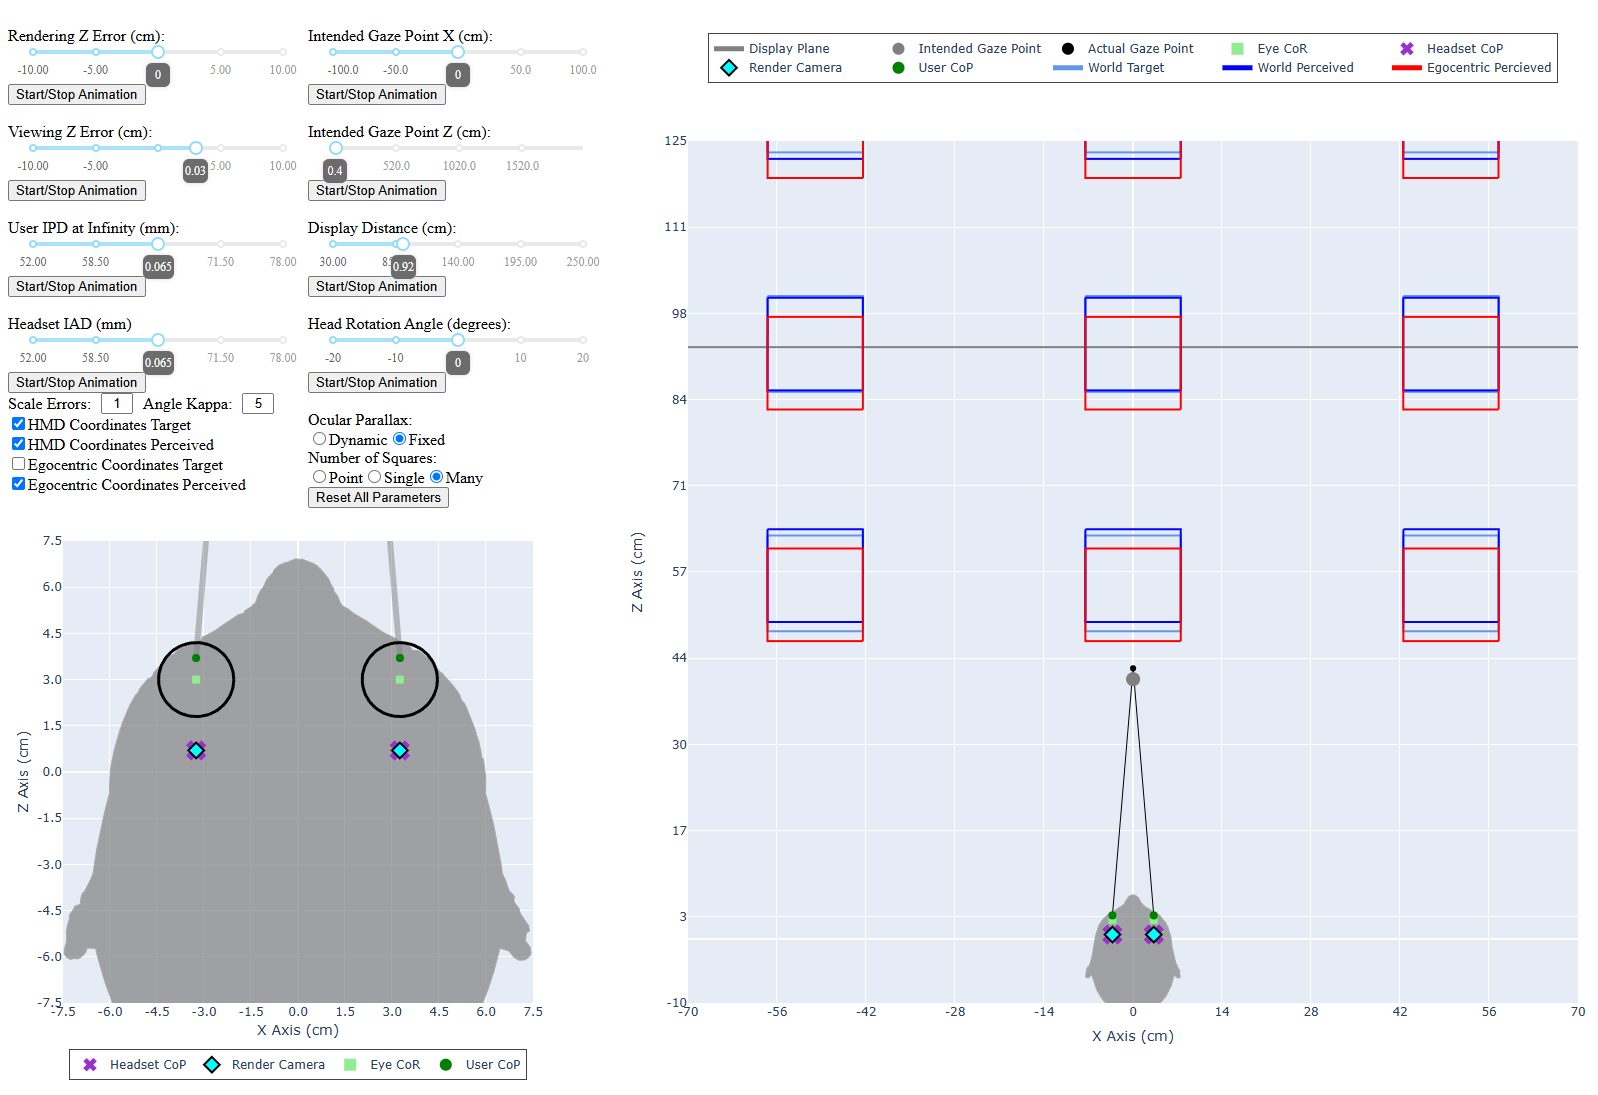
\includegraphics[width=\linewidth]{figures/model/webapp.png}    
	\caption{Interactive perspective stereo geometry visualizer provided in supplementary materials. In this simulation a viewing error moves the viewer 3 cm forward relative to the HMD coordinate system which leads to a 3 cm offset between the egocentric and HMD coordinate systems. This leads to potential discrepancies in conclusions about perceived distance if measurements taken in these two coordinate systems are directly compared. The intended render geometry in the HMD coordinate system is shown in light blue. The perceived geometry in HMD coordinate system according to perspective geometry is shown in dark blue. For viewing errors, objects on the virtual image plane are always perceived to be on the plane, according to stereo geometry. This means the center row of objects will appear near their intended position. However, because the viewer is closer to the display by 3 cm, this means that they will perceive the objects to be closer to them by 3 cm (boundaries in red) compared to the assumed HMD render geometry. This difference in coordinate systems can lead to seemingly paradoxical situations. For the row of objects closet to the user, the user will blind reach to the dark blue boundary, leading an external observer to think distance is overestimated (compared to light blue target). Yet the actual perception of the user is the red boundary and distance is in fact underestimated.} 
	\label{fig:geometric_model}
\end{figure*}

\begin{figure*}
	\centering
	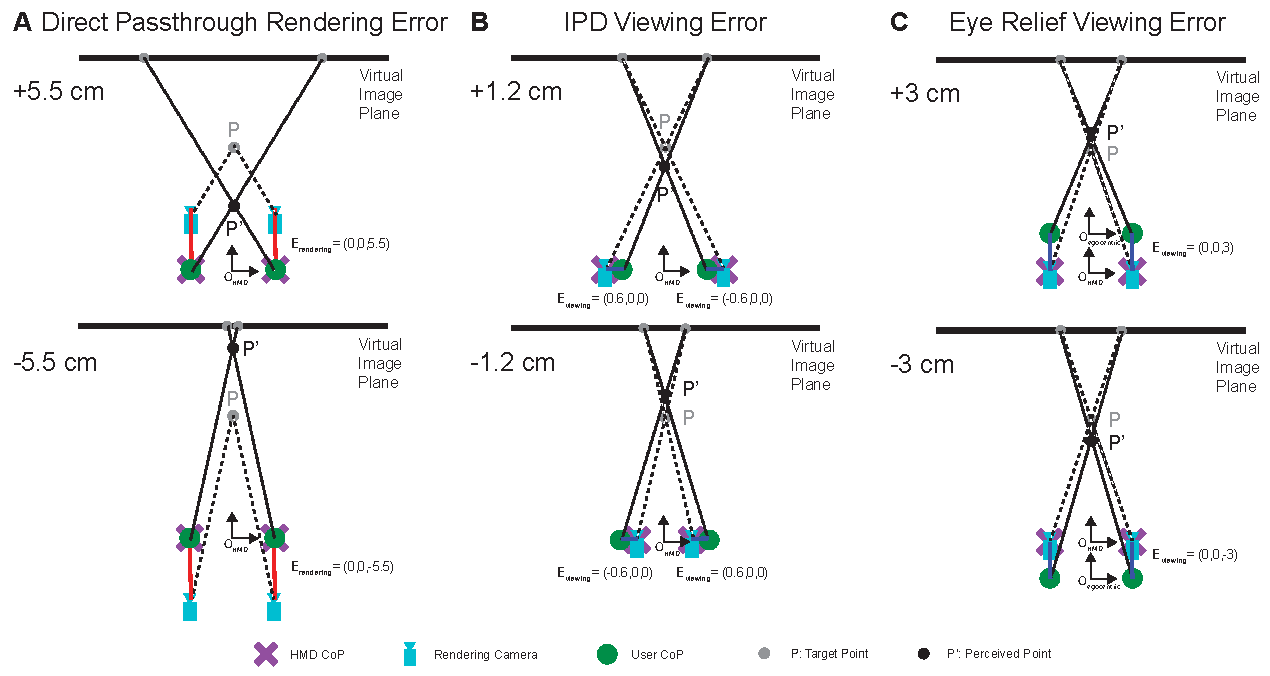
\includegraphics[width=\linewidth]{figures/reaching/error_choices.pdf}
	\caption{Rendering and viewing error conditions for the blind reaching experiments. \textbf{(A)} Direct passthrough rendering error results from showing images of cameras attached to the front of HMD without view reprojection. \textbf{(B)} IPD viewing error occurs when interaxial distance (IAD) of the HMD is smaller or larger than the user IPD. \textbf{(C)}. Eye relief viewing error is due to user's eyes being in front or behind the HMD CoP due to facial geometry. 
	}
	\label{fig:error_choices}
\end{figure*}


% \begin{figure*}
% 	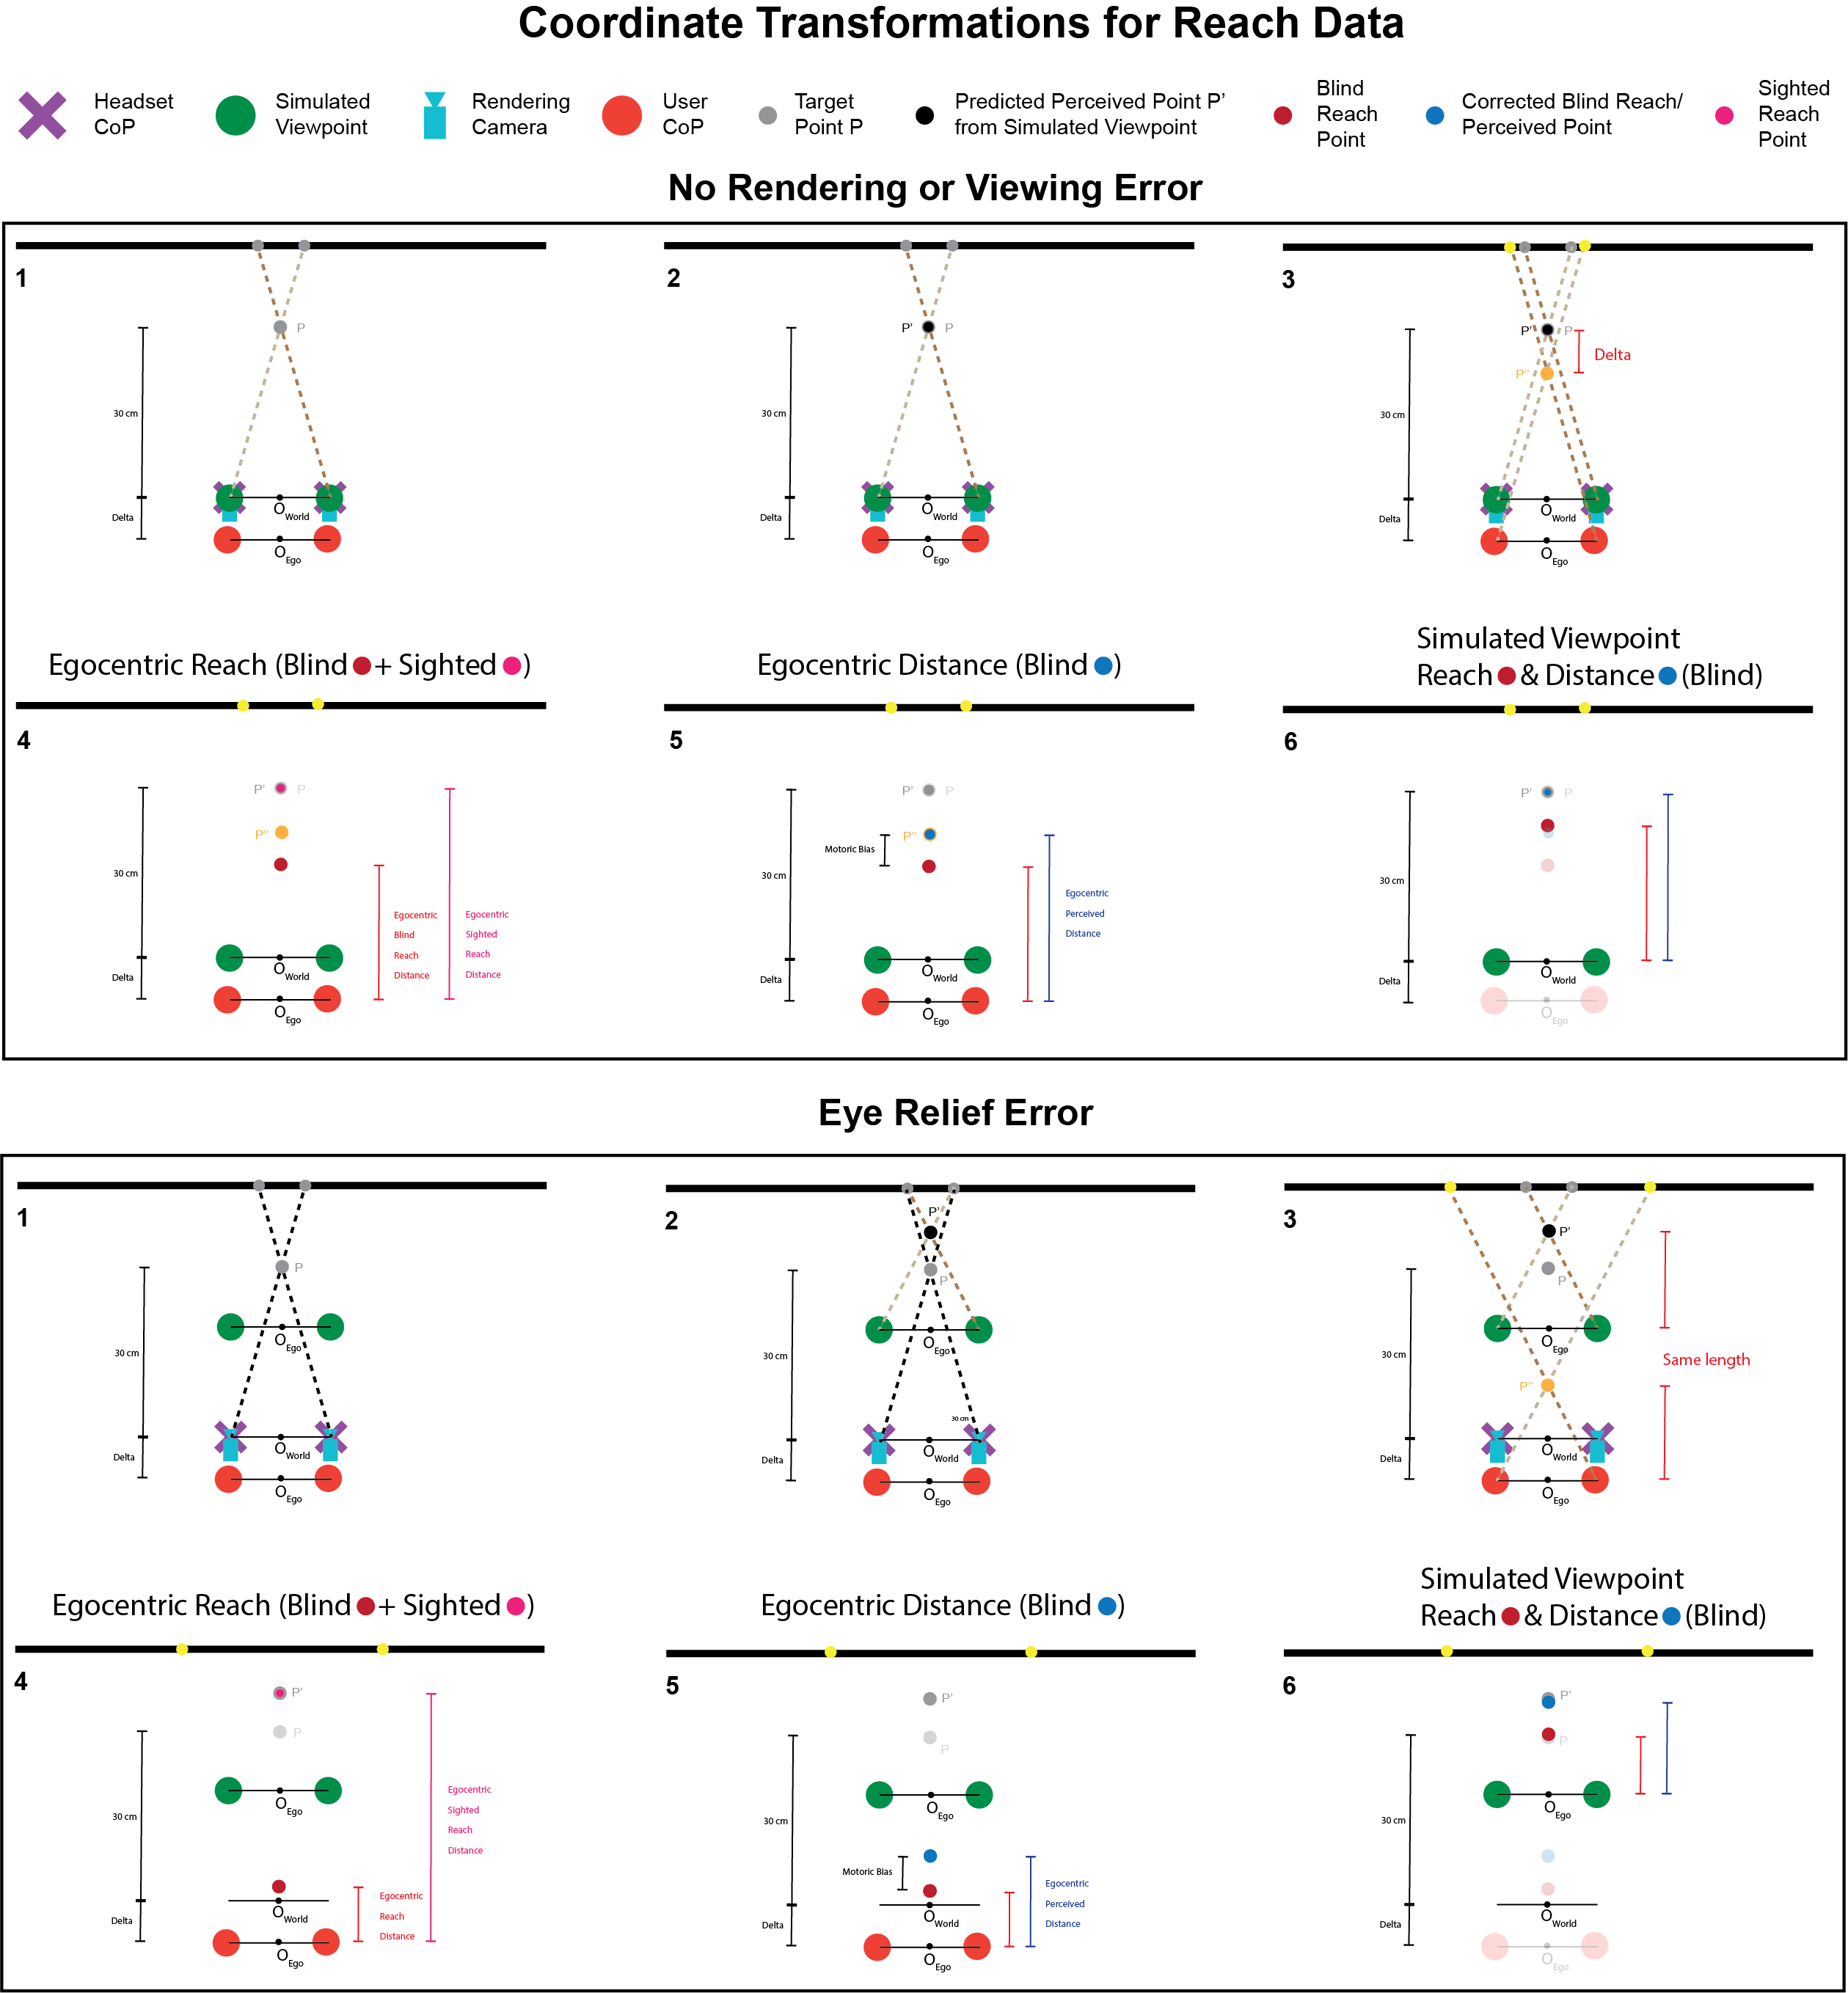
\includegraphics[width=1\textwidth]{figures/model/world_vs_egocentric_frame_step_by_step_combined.png}
%         \caption{Coordinate system transforms used to interpret reaching data studies. \textbf{(Top)} Our headset uses the largest Quest 3 eye relief setting available which results in an average eye relief viewing error of -12 mm. In panels 1-2 we show how a target point P is rendered at P' when no stereo geometry errors are added to the system. In panel 3 the rays used to simulated viewpoint are shown to the actual user who is slightly displaced away from the ideal eye relief resulting in a perceived point P'. In panels 4-6 we describe how sighted reaching, blind reaching, and bias-corrected blind reaching can be converted from measured values into their equivalent perceived values based on the small offset delta between the actual user eye position and simulated viewpoint. \textbf{(Bottom)} Simulated eye relief viewing errors require another transform to interpret egocentric reach data in the simulated viewpoint HMD coordinates which is shown in panels 5 and 6.}
% 	\label{fig:simulation_geometry}
% \end{figure*}

% \begin{figure*}
% 	\includegraphics[width=1\textwidth]{figures/model/distortion_field.png}
%         \caption{Geometric distortion fields in world coordinates at errors used in reaching experiments. \textbf{(A,B)} Direct passthrough errors. \textbf{(C,D)} Eye relief viewing error error. \textbf{(E,F)} mismatched IPD-IAD errors. For viewing errors (C-F), points on the virtual image plane are not distorted. For rendering errors (A-B), distortions are the same irrespective of virtual image plane distance.}
% 	\label{fig:distortion_vector_field_summary}
% \end{figure*}


\end{document}